\documentclass[../tp3_grupo404.tex]{subfiles}

\graphicspath{{\subfix{../out/}}}

\begin{document}

Para la solución al problema planteado se propone reducir el problema a un problema de corte de flujo
y solucionarlo con el algoritmo de Edmonds-Karp.

\begin{figure}[H]
    \centering
    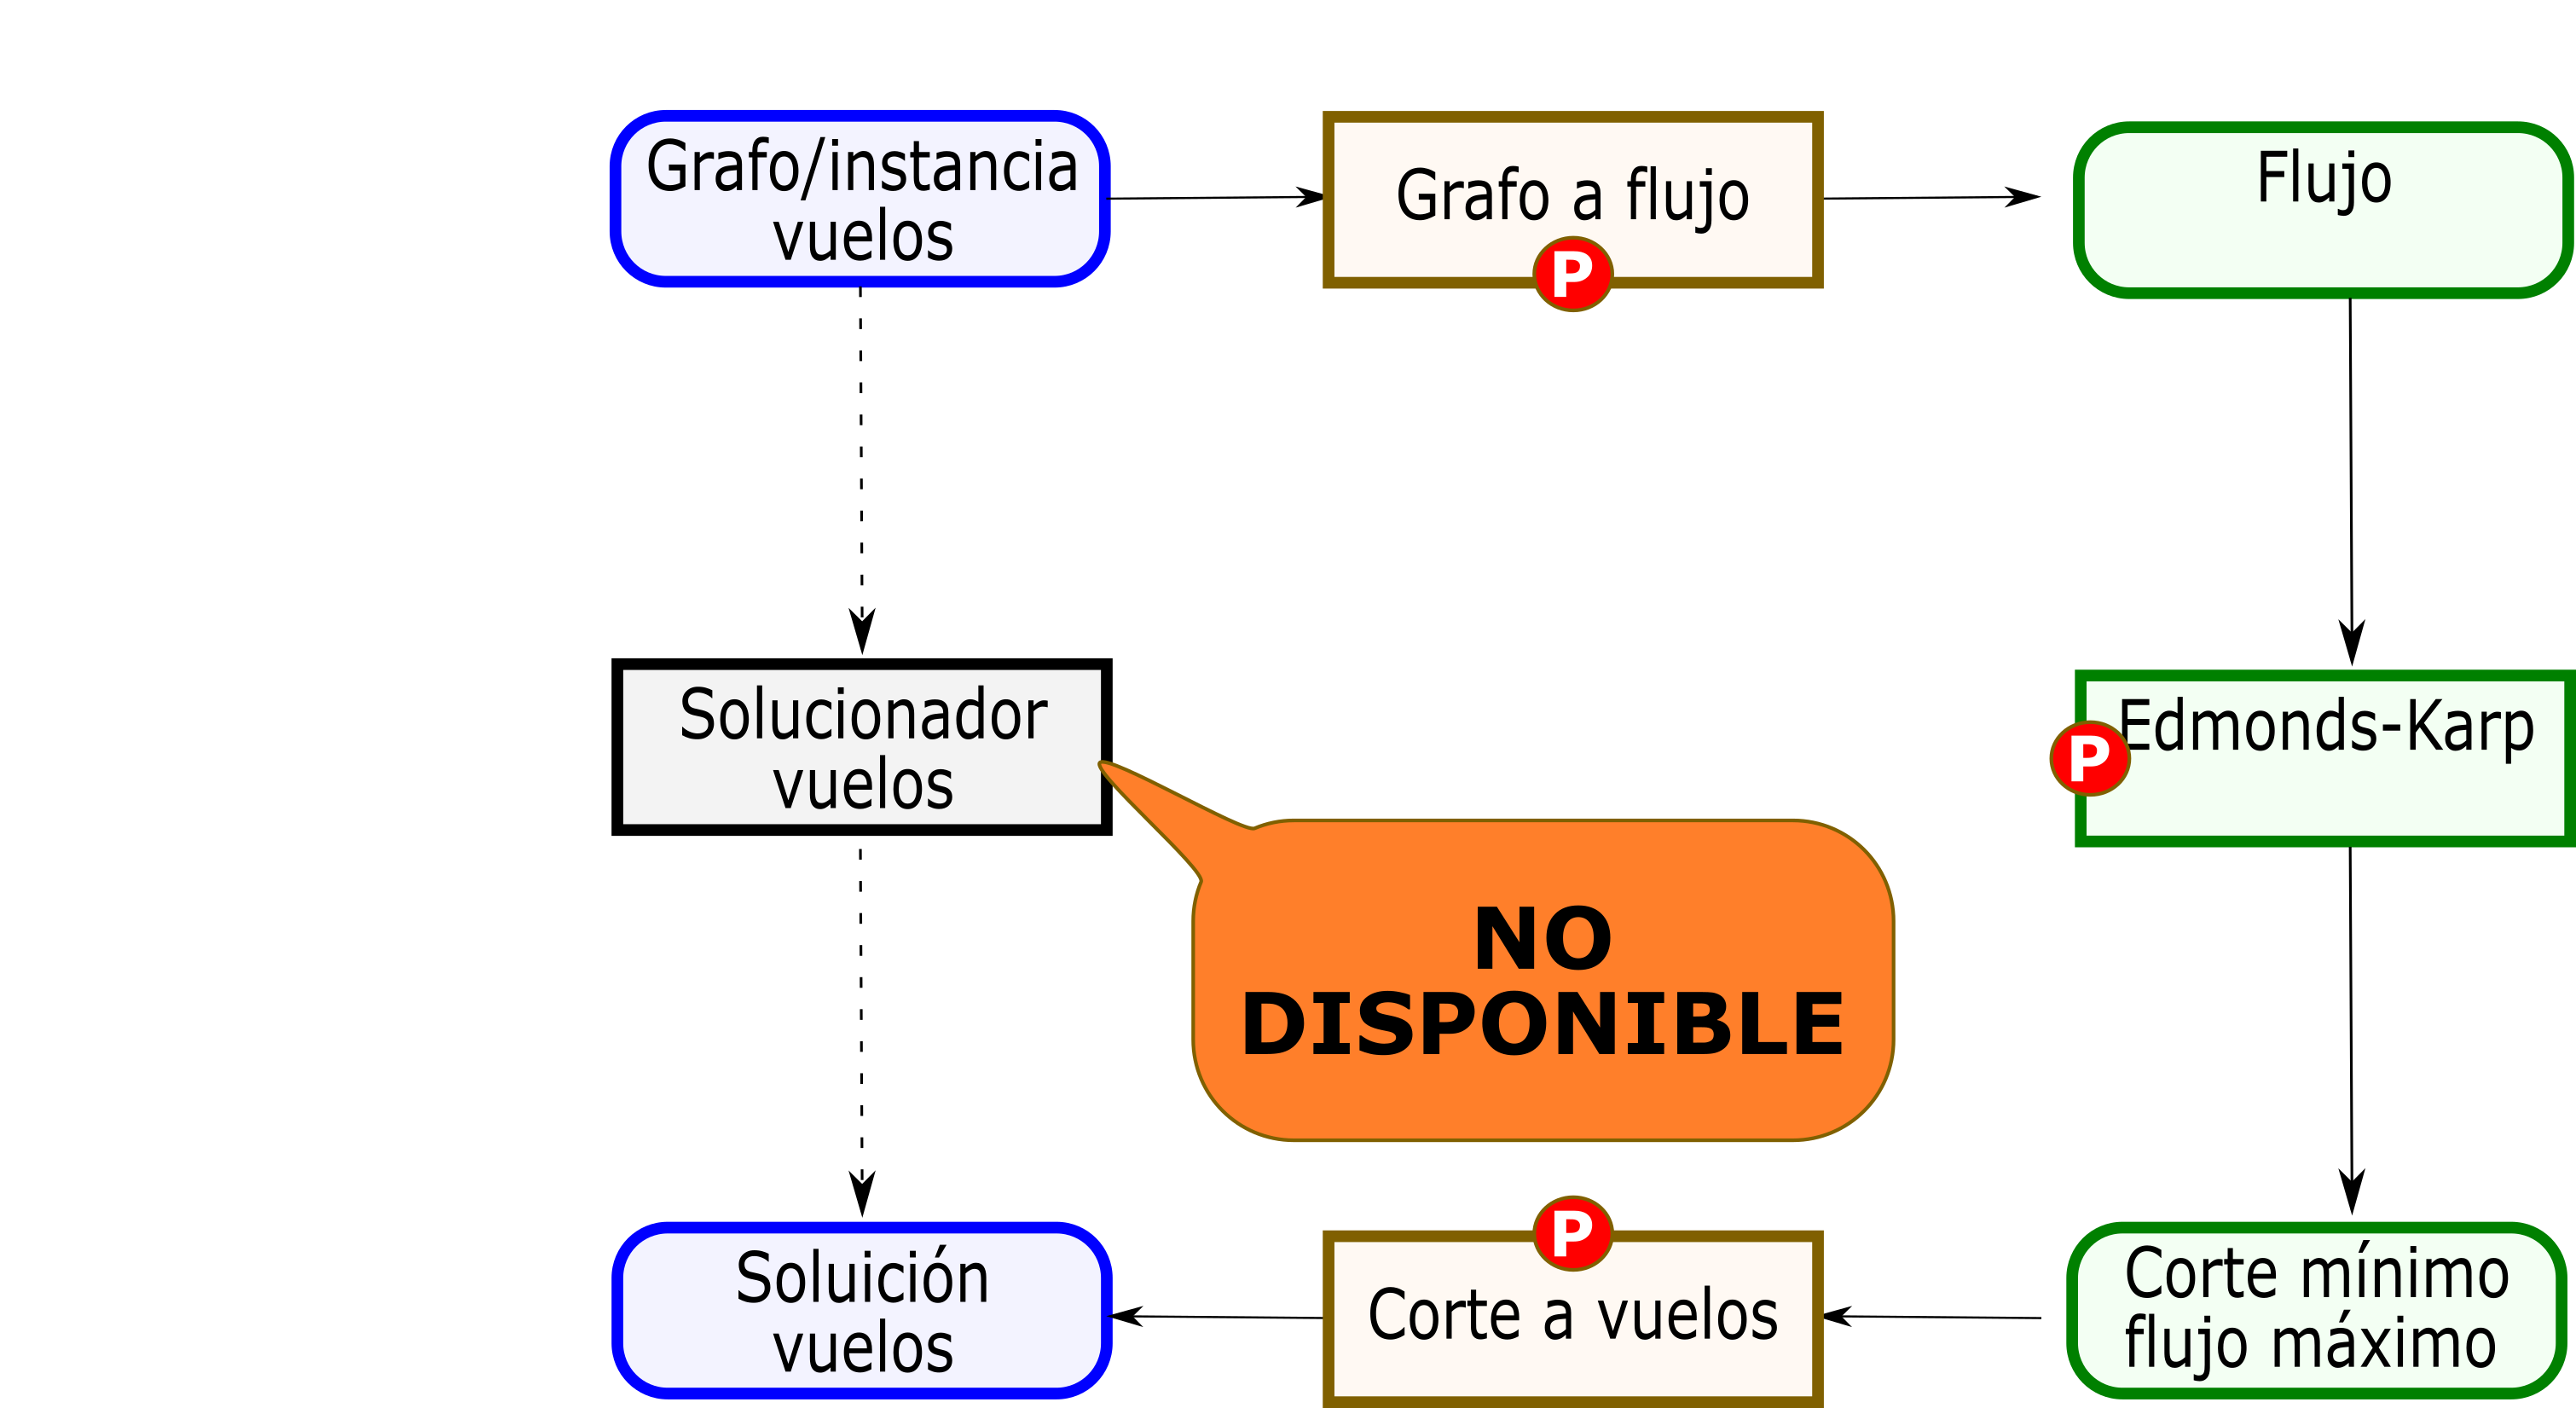
\includegraphics[width=0.9\linewidth,angle=0,origin=c]{out/reduc.png}
    \caption{\label{reduc}Reducción del problema, todas las operaciones son polinómicas.}
\end{figure}

\subsubsection{Pasos generales}

En resumen, la solución completa sigue los siguientes pasos:
\begin{enumerate}
    \item Procesar el archivo en el formato dado a un grafo dirigido, utilizando lista de adyacencias.
    \begin{itemize}
        \item Cada nombre de aeropuerto es tratado como un número indicando la posición, en la lista
        de adyacencias, de cada lista de destino para un mismo origen.
        \item Cada elemento está compuesto por una tupla de id de destino y "peso" asociado.
        \item La estructura permite que peso pueda no ser simplemente un número, y el alias puede no ser un string.
            Pero en este punto, por el formato de entrada, sí lo serán.
    \end{itemize}
    \item Convertir el grafo en un diagrama de flujo, en el que:\begin{itemize}
        \item En cada arco original se almacena:\begin{itemize}
            \item una \textbf{capacidad máxima}, cuyo valor está dado por el anterior peso numérico del grafo.
            \item y un \textbf{flujo}, incialmente 0 (cero).
        \end{itemize}
        \item Cada arco original (a través de la clase \texttt{ArcoDirecto}) se obtiene un valor dado por
            la capacidad residual (la capacidad - el flujo). En el sentido contrario del grafo se almacena
            una referencia (a través de \texttt{ArcoInverso}) que, como valor, devuelve el flujo del arco
            directo (en el sentido original).
            \par Por ejemplo, un arco $A\underset{10}{\rightarrow}B$ es reemplazado por un ArcoDirecto
            $A\underset{0/10}{\rightarrow}B$ que devuelve un valor $10-0=0$, y se agrega un nuevo arco
            $B\rightarrow A$ (que referencia al anterior) y devuelve un valor igual al flujo ($0$).
    \end{itemize}
    \item Se aplica Edmonds-Karp: \begin{enumerate}
        \item Se inicializa en 0 un contador interno de flujo aumentado.
        \item Mientras haya un camino, encontrado con BFS, desde el origen y el destino dados en el archivo,
        cuyos arcos tengan valores mayores que cero:\footnote{Esto es, para un arco directo significa que
        hay un valor residual, el flujo no llegó a su capacidad máxima. para un arco inverso significa que
        hay un flujo en el sentido contrario que podría disminuirse.} \begin{enumerate}
            \item  Busca el cuello de botella (el menor de todos los valores).
            \item Aumenta el camino: Si es un arco directo, aumenta el flujo (reduciendo su "valor" y
            aumentando el del arco inverso asociado); si es un arco inverso, disminuye su flujo (aumentando
            su "valor", y reduciendo el del arco directo, ya que es el valor residual).
            \item Se aumenta un contador interno de flujo aumentado con el valor del cuello de botella.
        \end{enumerate}
    \end{enumerate}
    \item Al terminar, se recorre con un BFS todos los nodos a los que pueda llegarse por un arco no saturado,
        es decir donde no haya un valor directo de 0 (si lo hay se lo agrega aun subconjunto de arcos \texttt{corte}),
        y se los agrega al subconjunto A; el resto de los nodos pertenecen al subconjunto B.
    \item Se devuelve el contador de flujo como capacidad máxima de pasajeros del origen al destino,
    y el conjunto de arcos \texttt{corte} como los vuelos que cumplen con el criterio dado.
\end{enumerate}

\subsubsection{Ejemplo}
Tomaremos como ejemplo el archivo disponible en
\texttt{tests/entradas/test\_ejtp3.txt}. En la línea 1 y 2 tenemos el origen y
destino (respectivamente) de los pasajeros a los que apunta la campaña.
Y a continuación, en el epígrafe de cada figura, iremos desarrollando el ejemplo.

\begin{alternate}[breaklines=true,numbers=left,xleftmargin=5mm]
    BHI
    MDZ
    AEP,MDZ,10
    BHI,MDQ,20
    BHI,NQN,11
    EZE,AEP,15
    MDQ,EZE,18
    NQN,AEP,11
    NQN,ROS,12
    ROS,MDZ,10
\end{alternate}

\begin{figure}[H]
    \centering
    \subcaptionbox
        {\label{fig:Vuelos1}\textbf{Grafo inicial con vuelos y sus capacidades}}
        {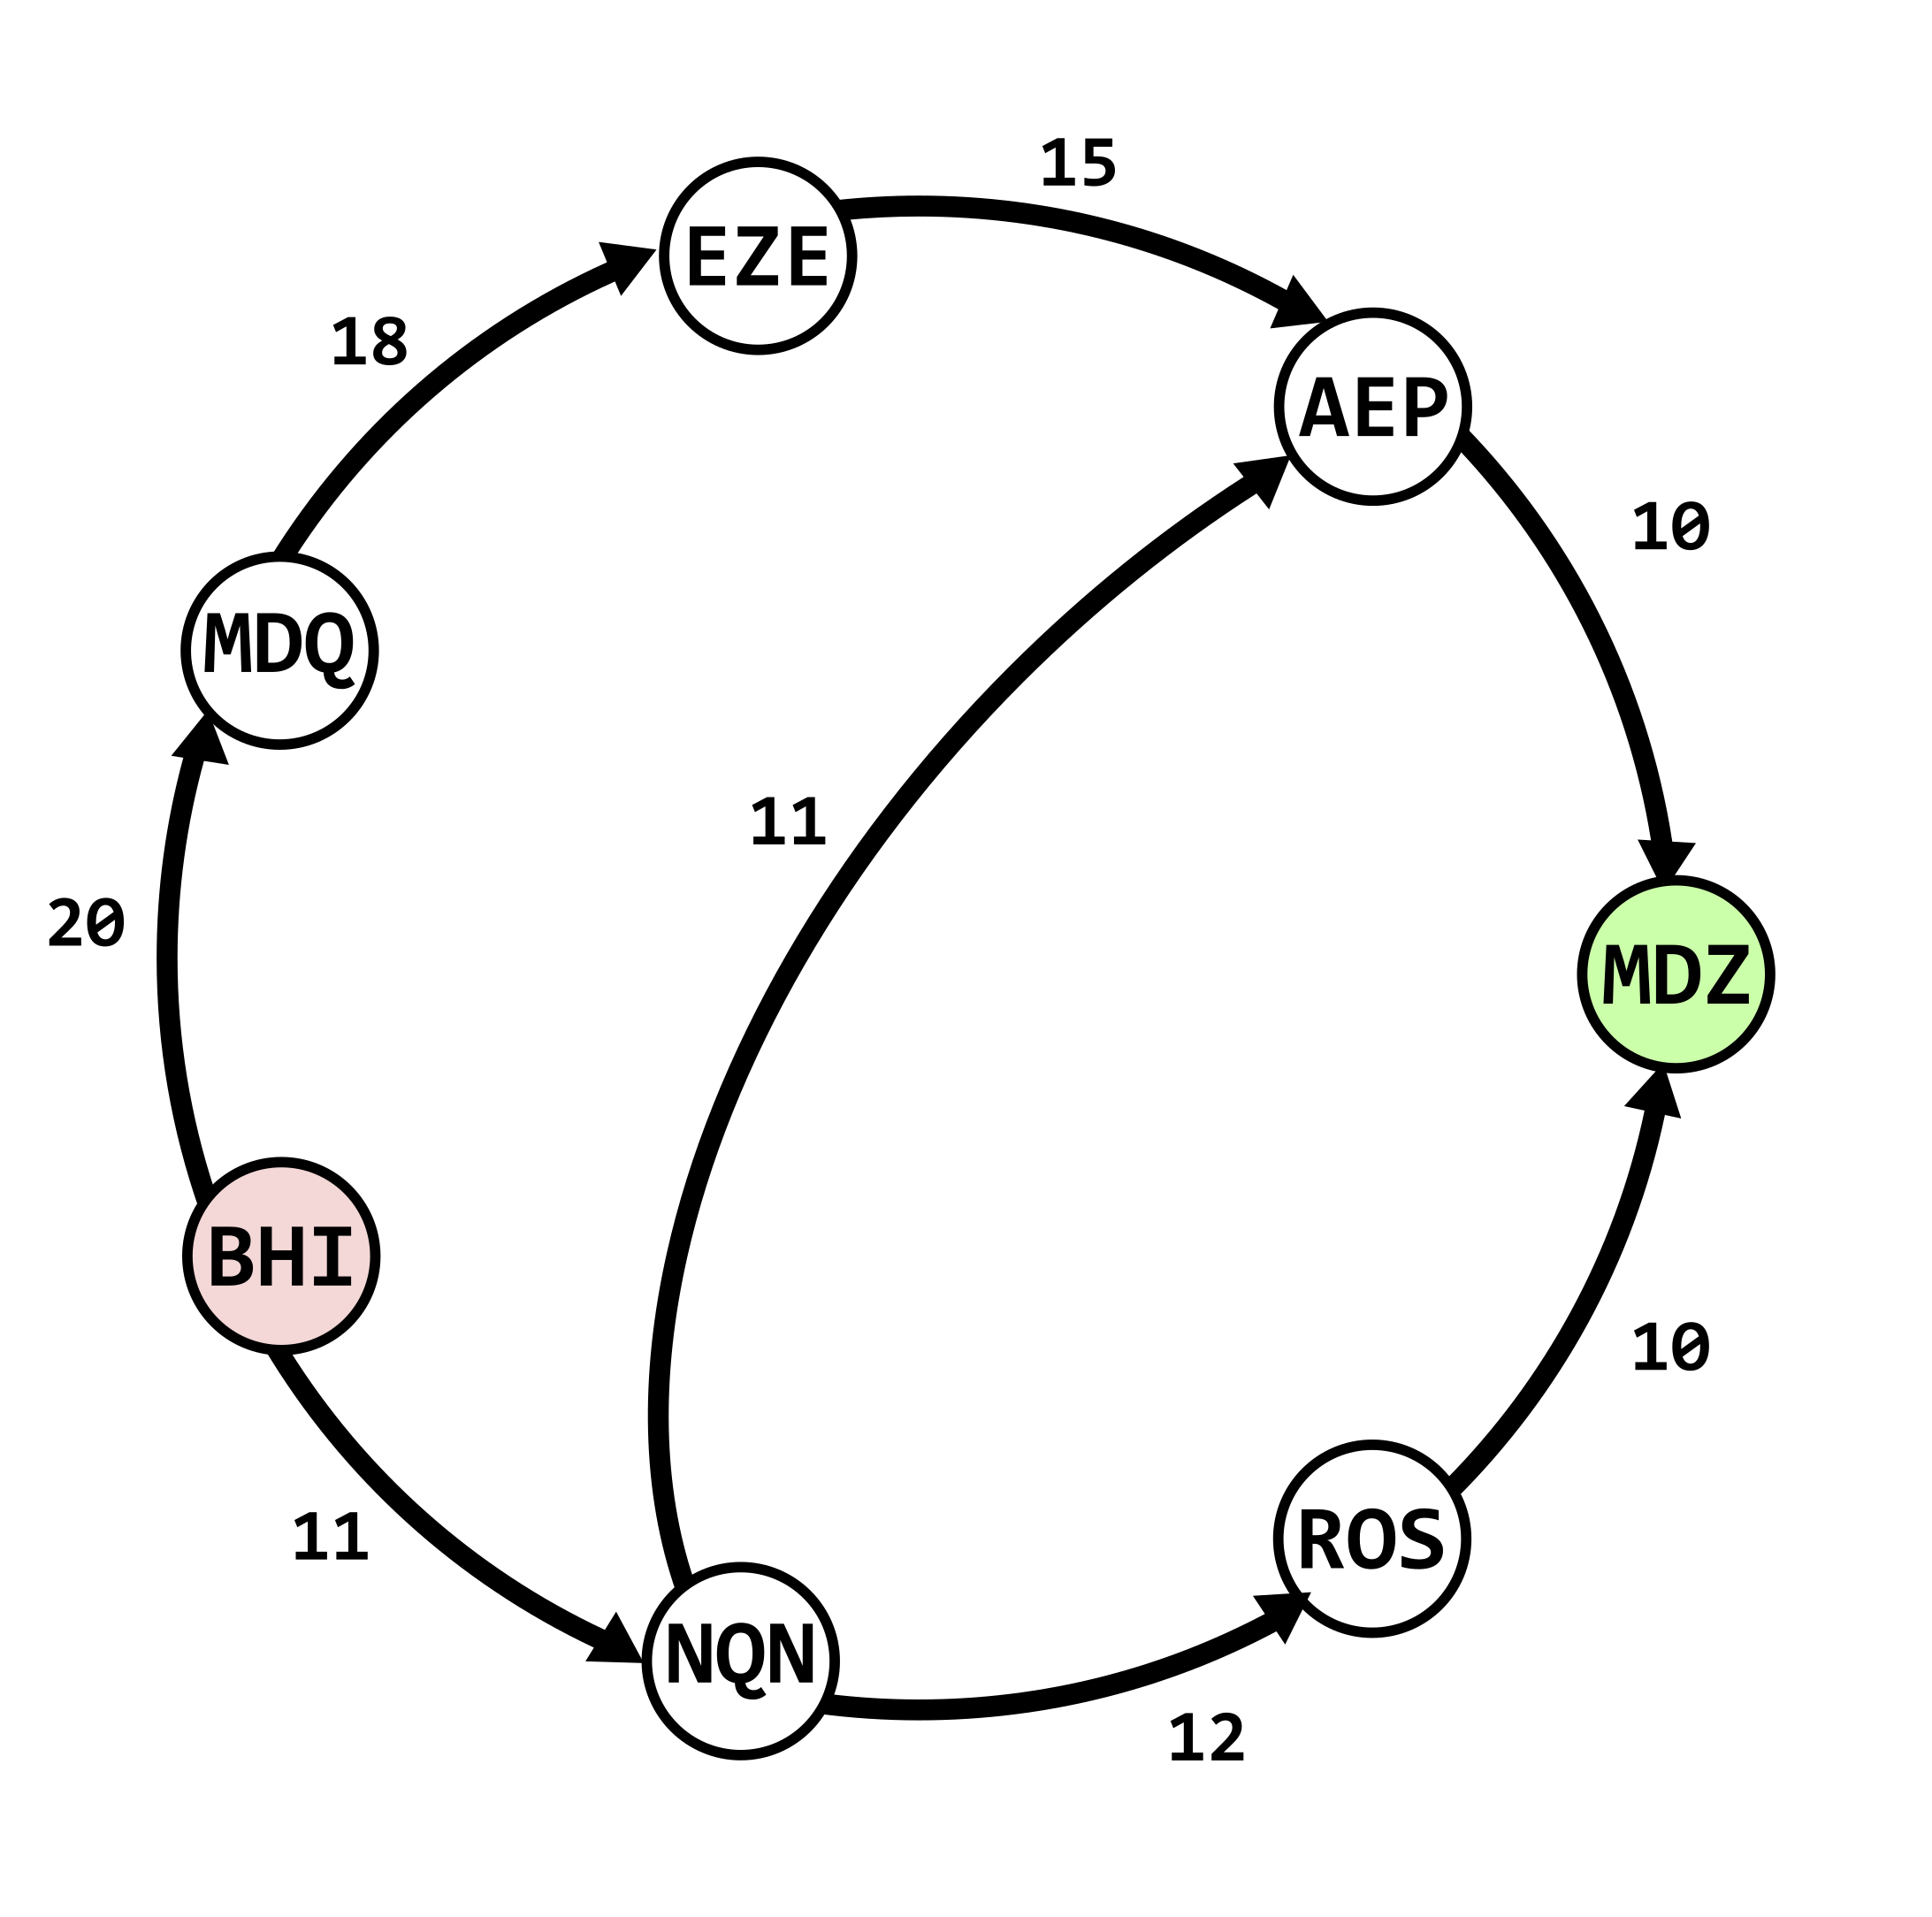
\includegraphics[width=0.4\linewidth,angle=0,origin=c]{out/ejA1.png}}
    \subcaptionbox
        {\label{fig:Vuelos2}\textbf{Conversión a grafo residual de flujo}, inicialmente flujo 0
        (flecha intermitente) y residuo disponible igual a su capacidad (felcha sólida).}
        {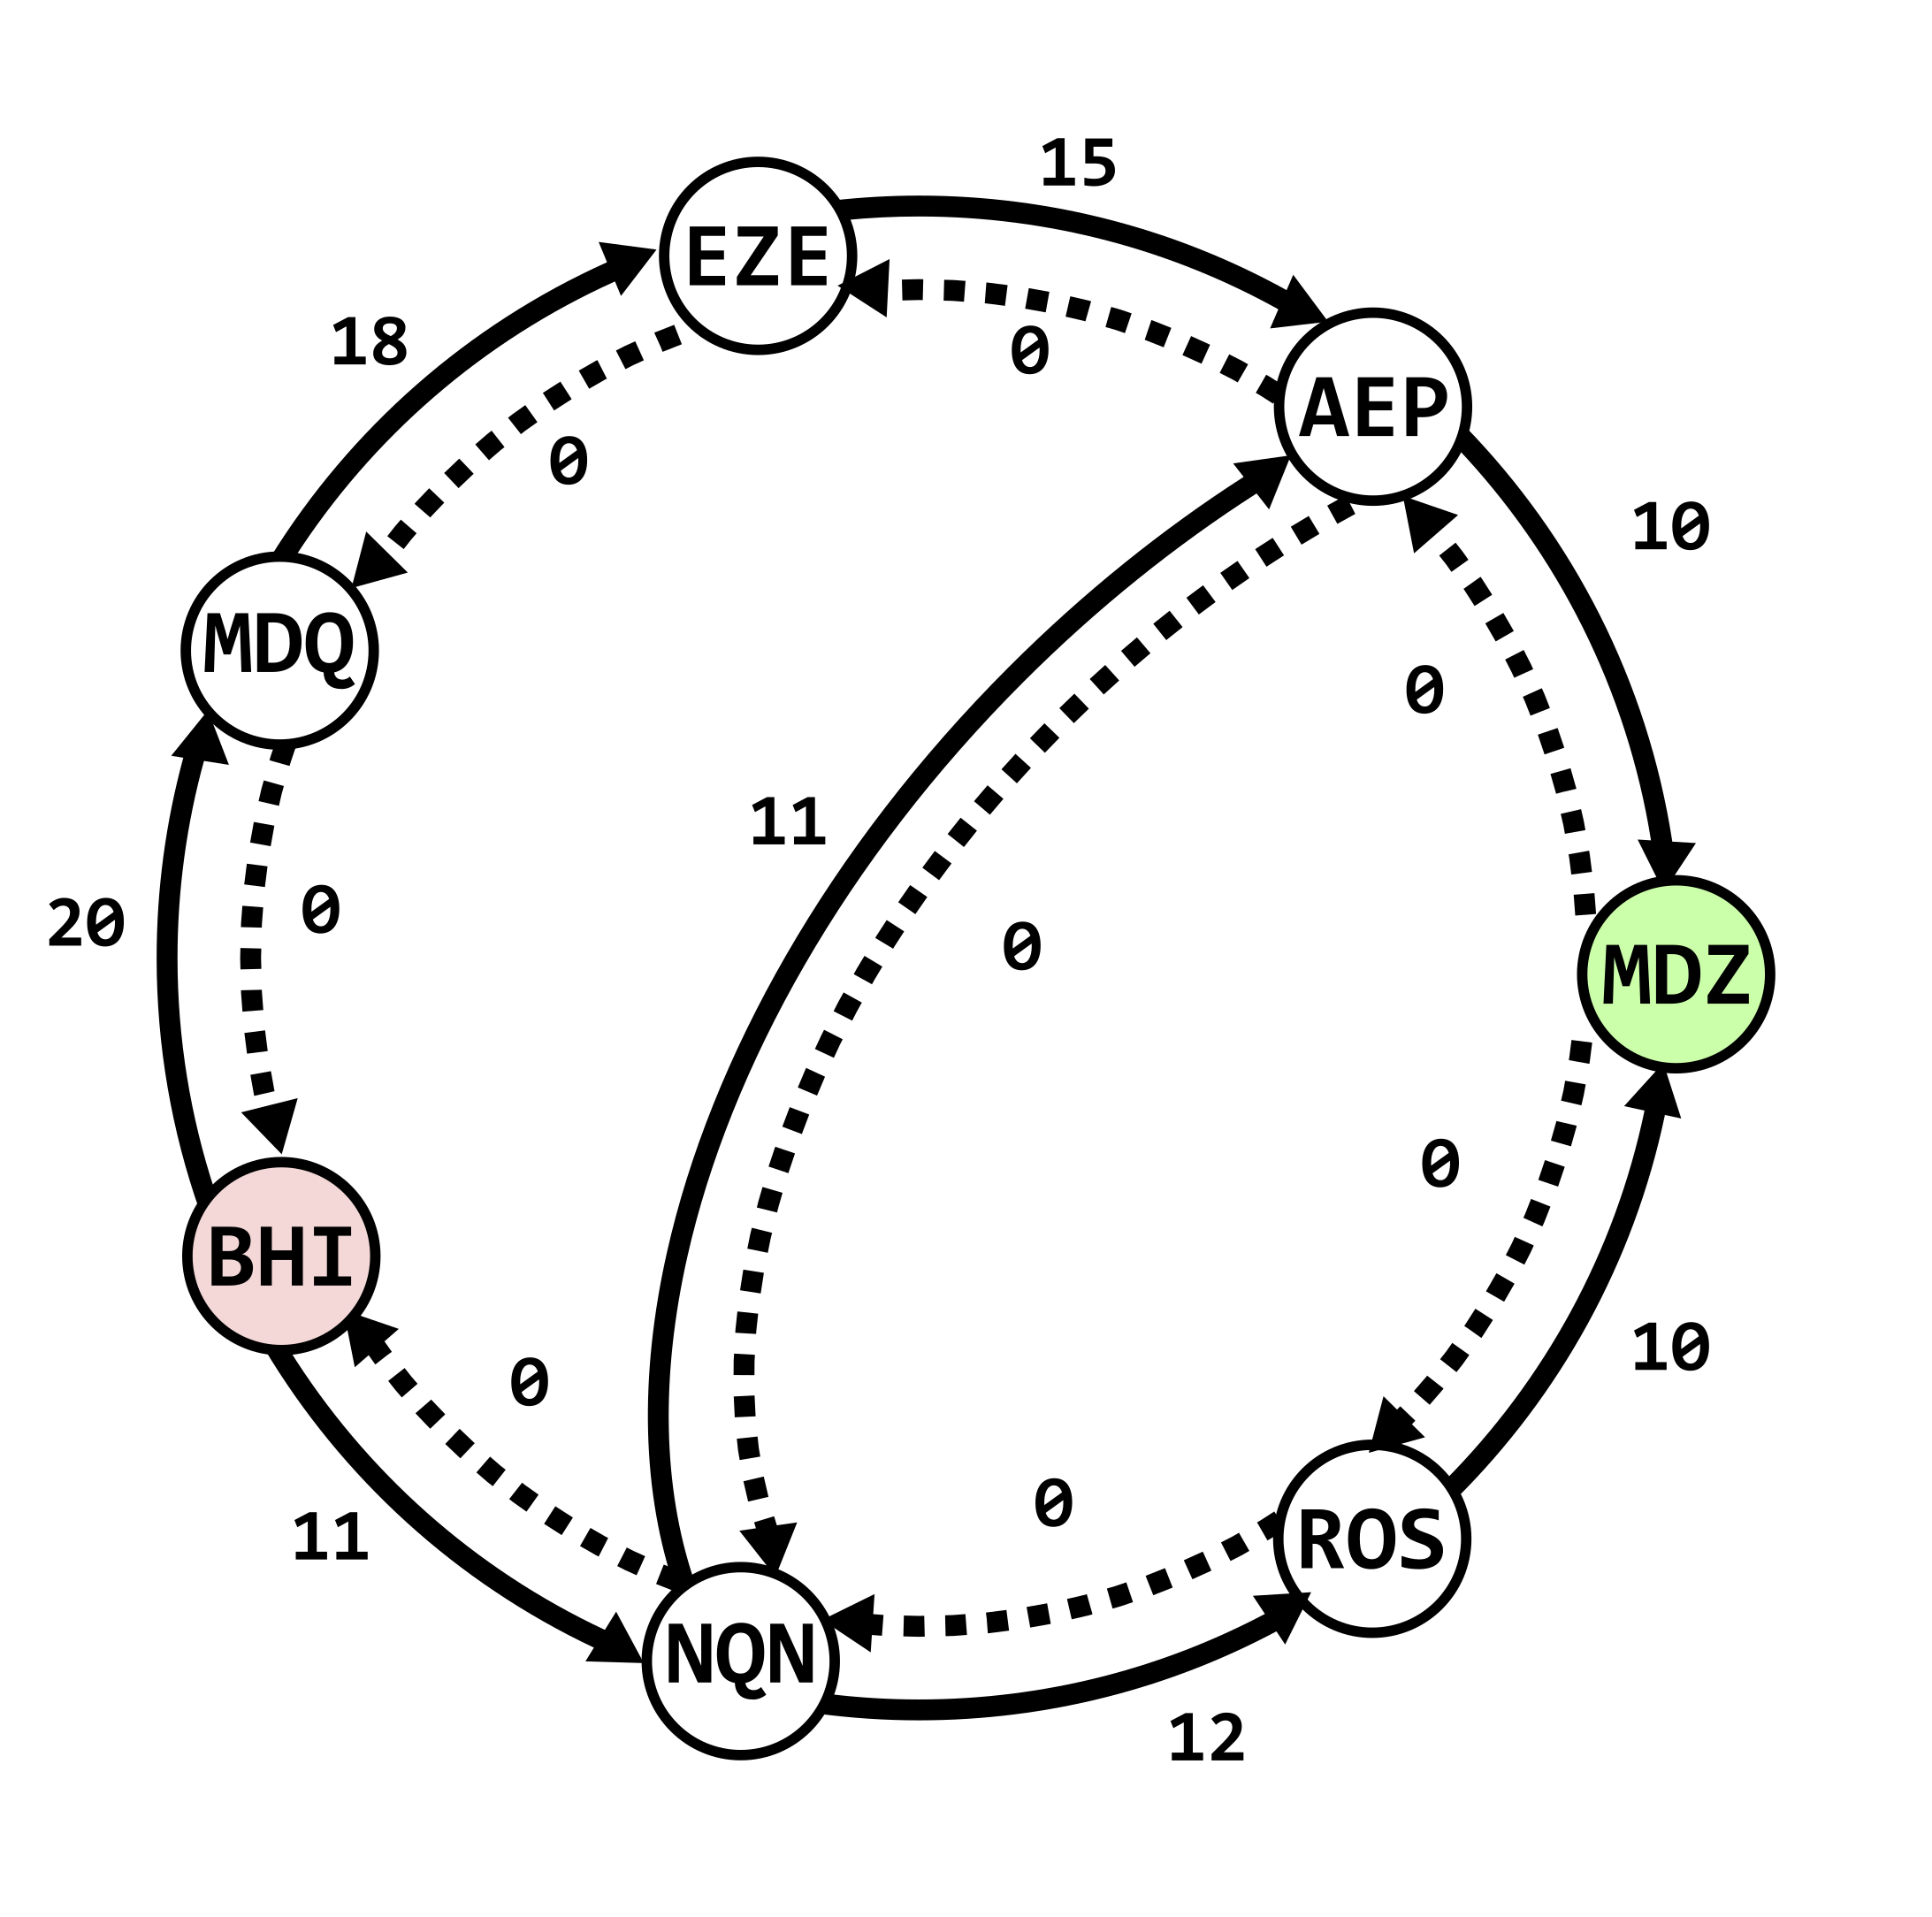
\includegraphics[width=0.4\linewidth,angle=0,origin=c]{out/ejA2.png}}
\end{figure}
\begin{figure}[H]
    %\ContinuedFloat
    \centering
    \subcaptionbox
        {\label{fig:Vuelos3}\textbf{BFS:} Hay varios caminos disponibles, puntualmente 2 mínimos (rojo y azul).
        Tomaremos el rojo con un cuello de botella de 10.}
        {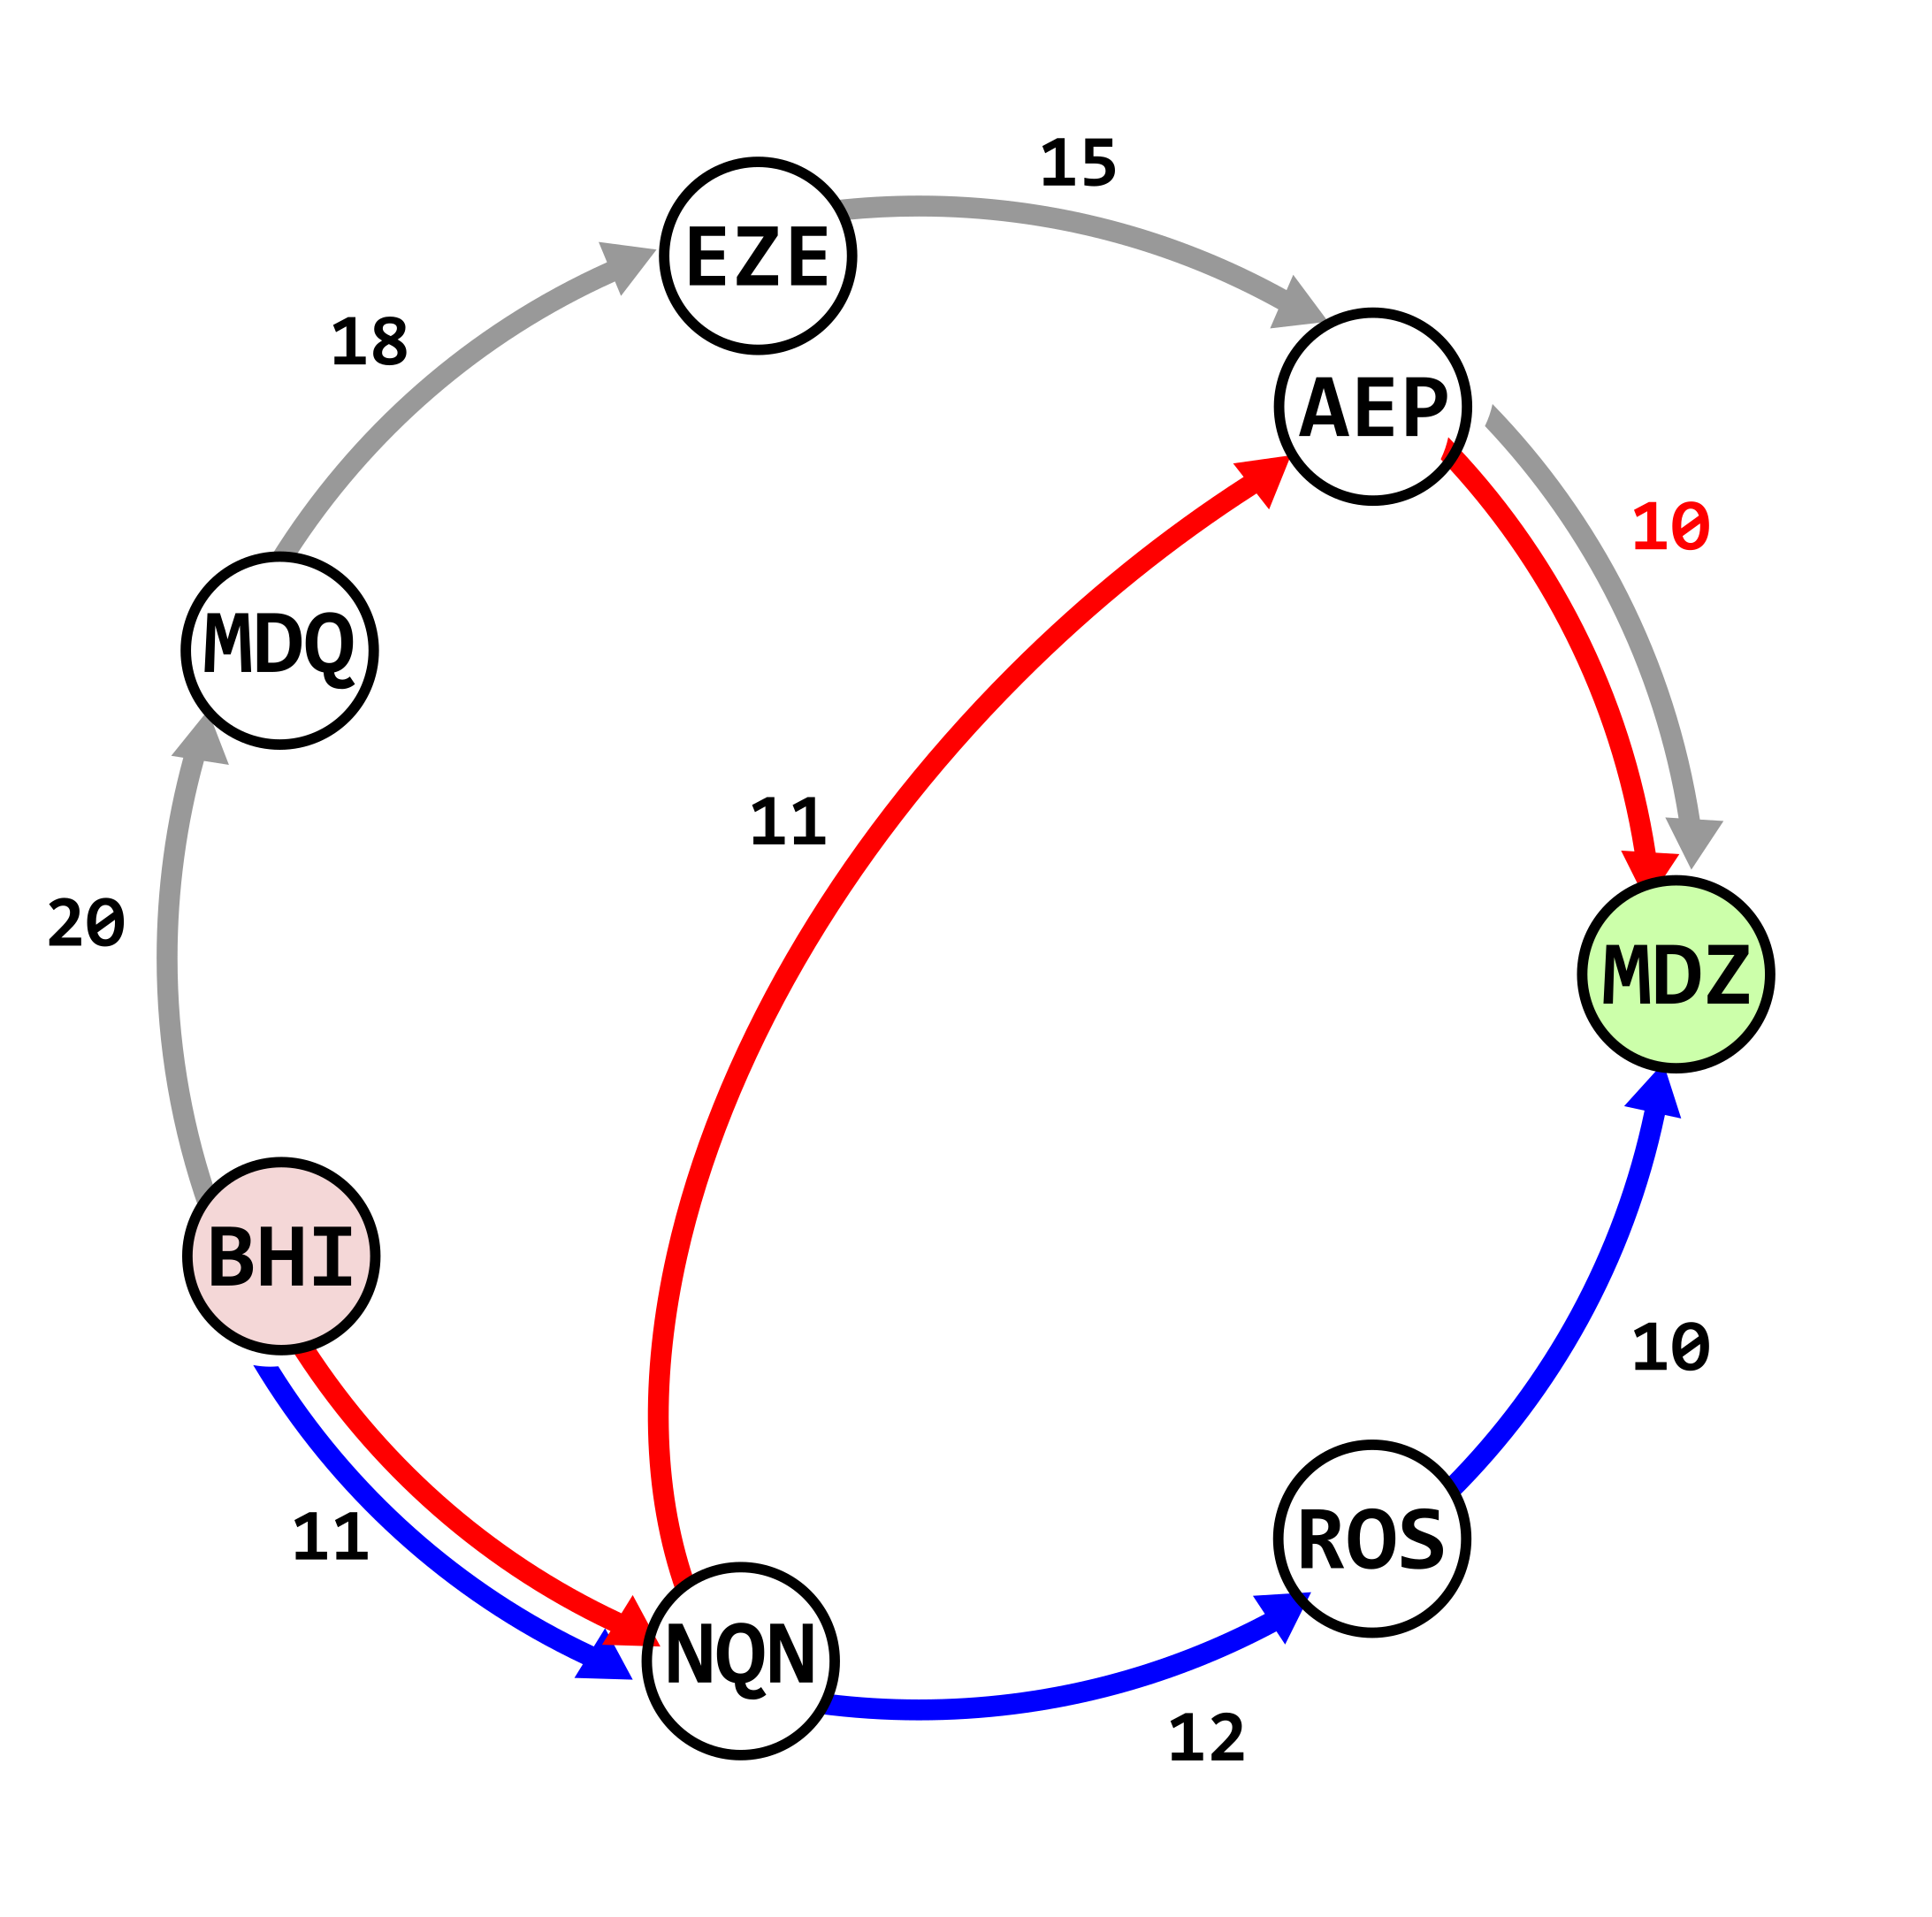
\includegraphics[width=0.4\linewidth,angle=0,origin=c]{out/ejA3.png}}
    \subcaptionbox
        {\label{fig:Vuelos4}\textbf{Aumentar:} A cada arco en sentido del camino se le resta el cuello (10, en ),
        y a cada arco en sentido contrario se le suma (manteniéndose la capacidad). El flujo total queda en 10.}
        {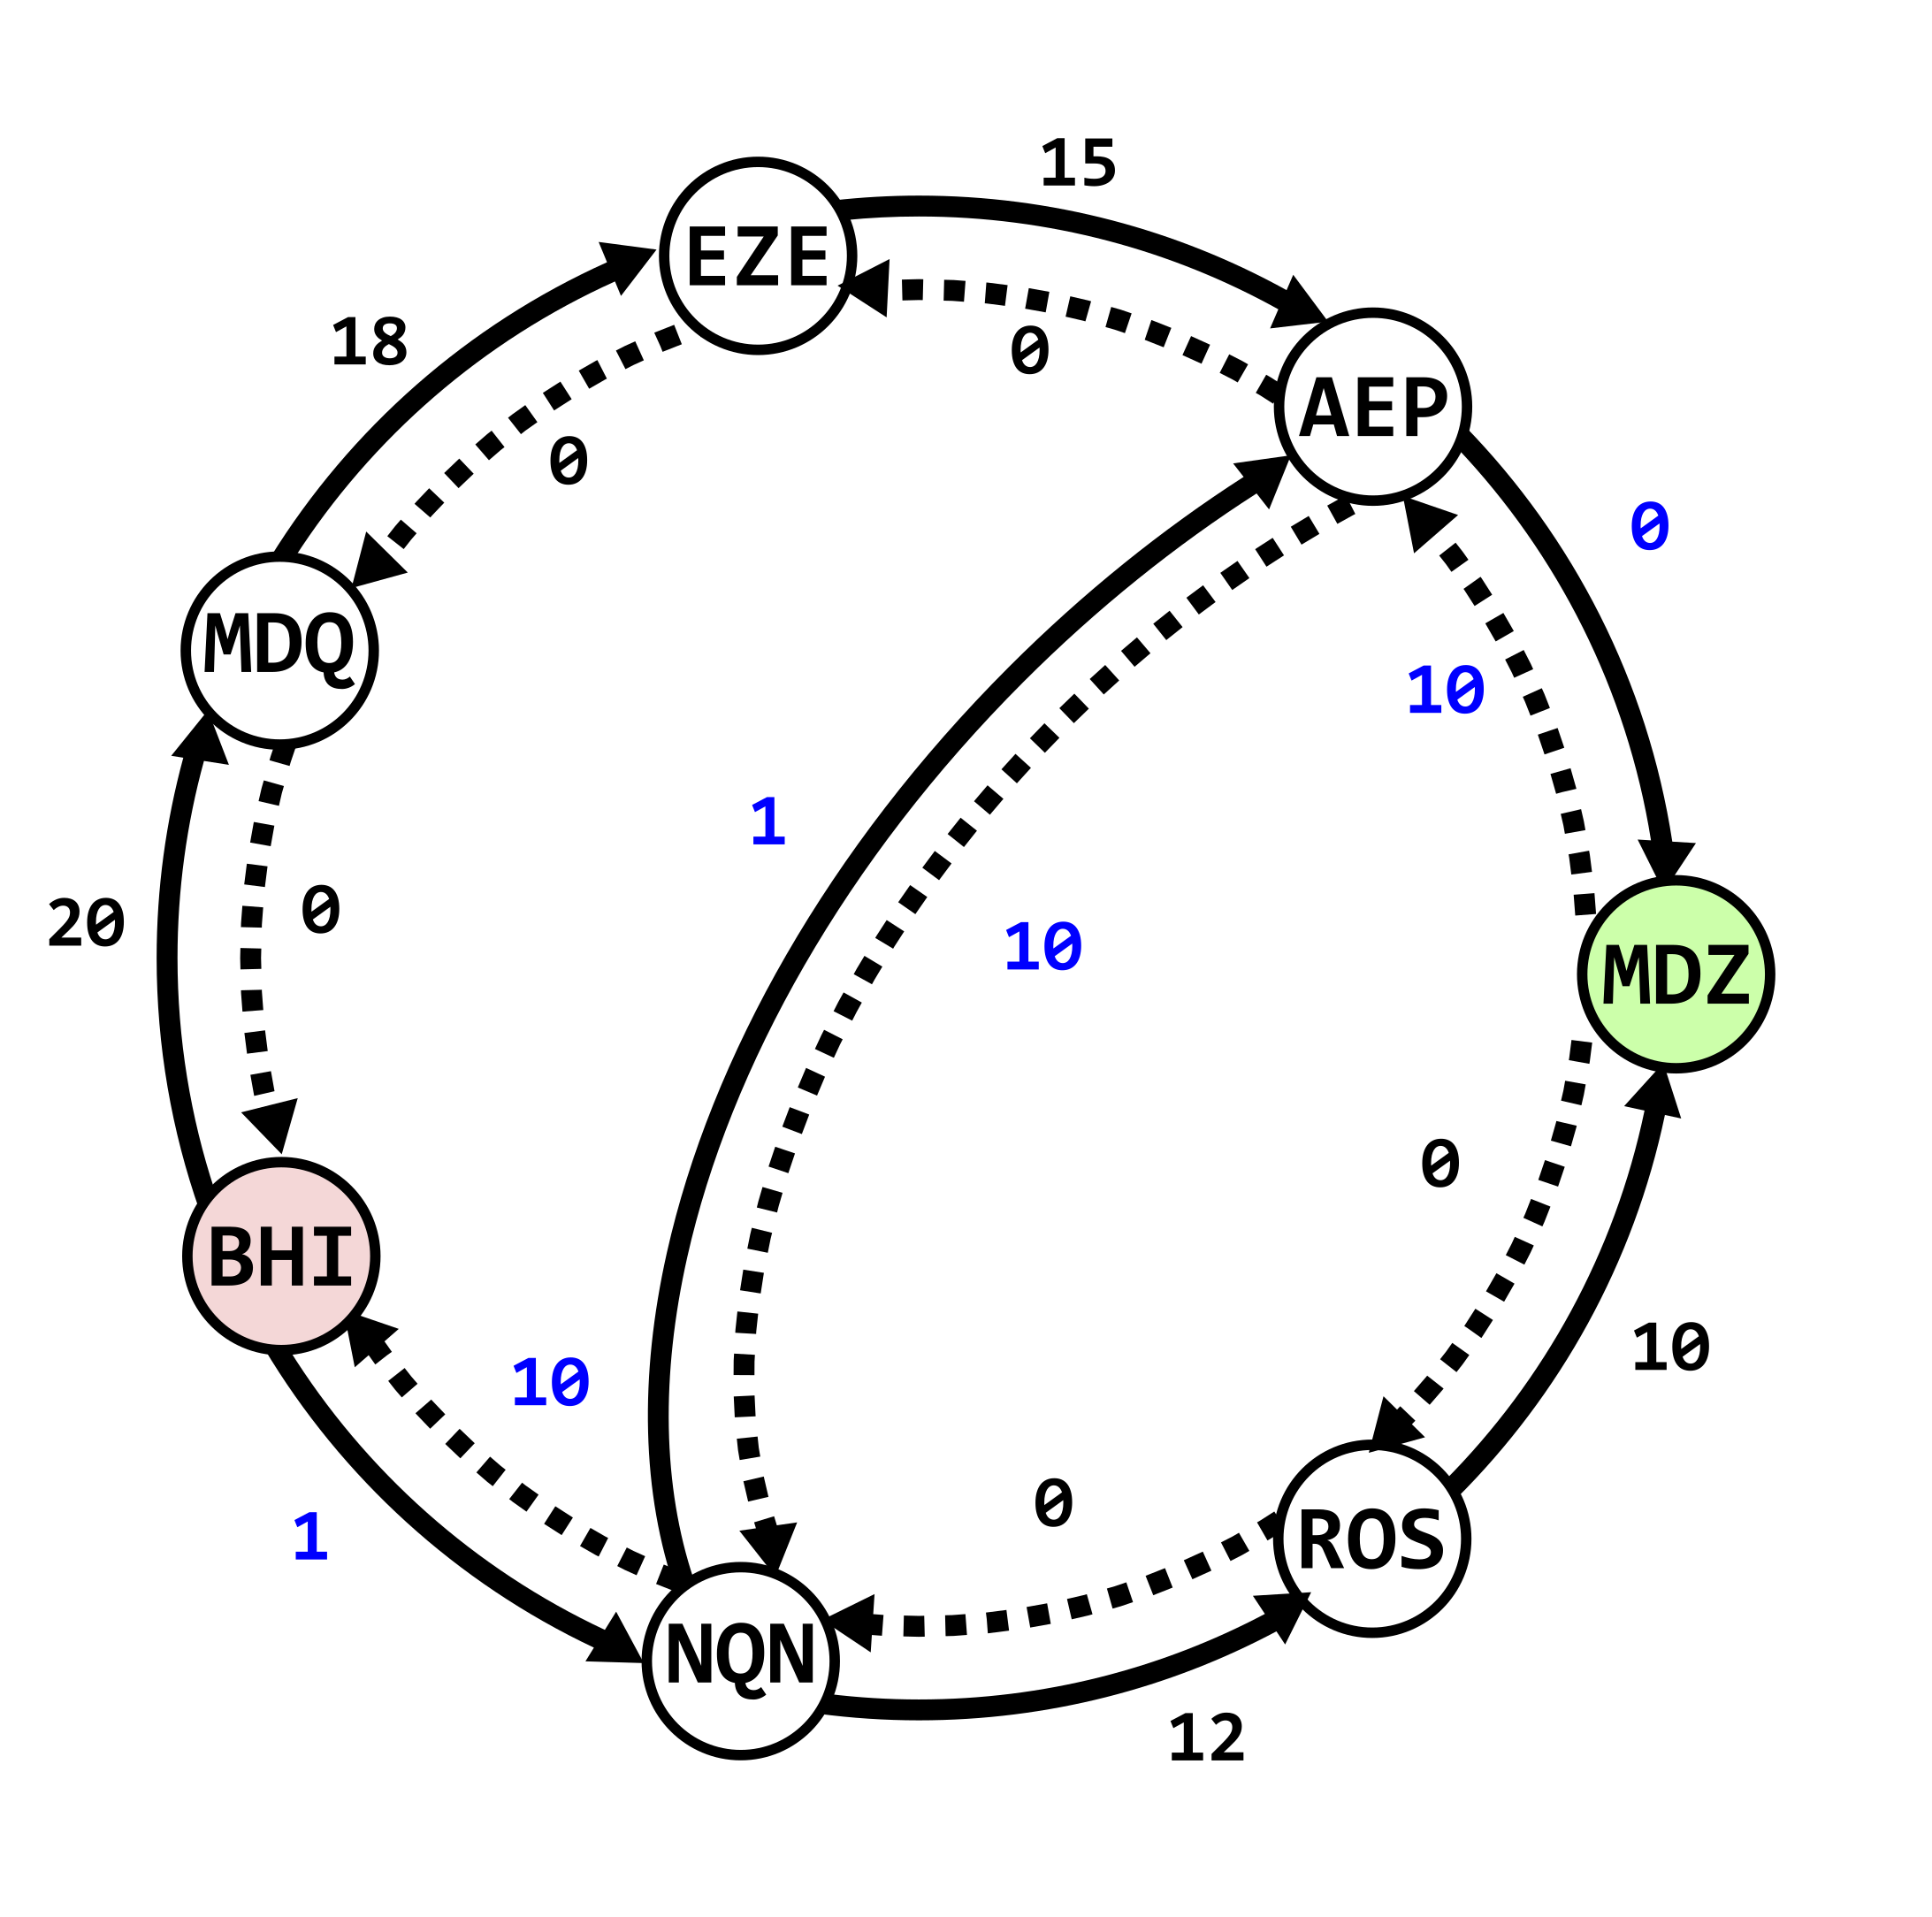
\includegraphics[width=0.4\linewidth,angle=0,origin=c]{out/ejA4.png}}
    \end{figure}
    \begin{figure}[H]
        %\ContinuedFloat
    \centering
    \subcaptionbox
        {\label{fig:Vuelos5}\textbf{BFS:} El siguiente camino mínimo es el indicado en rojo. El camino anterior
        ya no está disponible porque tiene al menos un arco ($AEP\rightarrow MDZ$) en 0. Siendo camino directo
        significa que no hay residuo, está saturado. El cuello de botella es 1 ($BHI\rightarrow NQN$).}
        {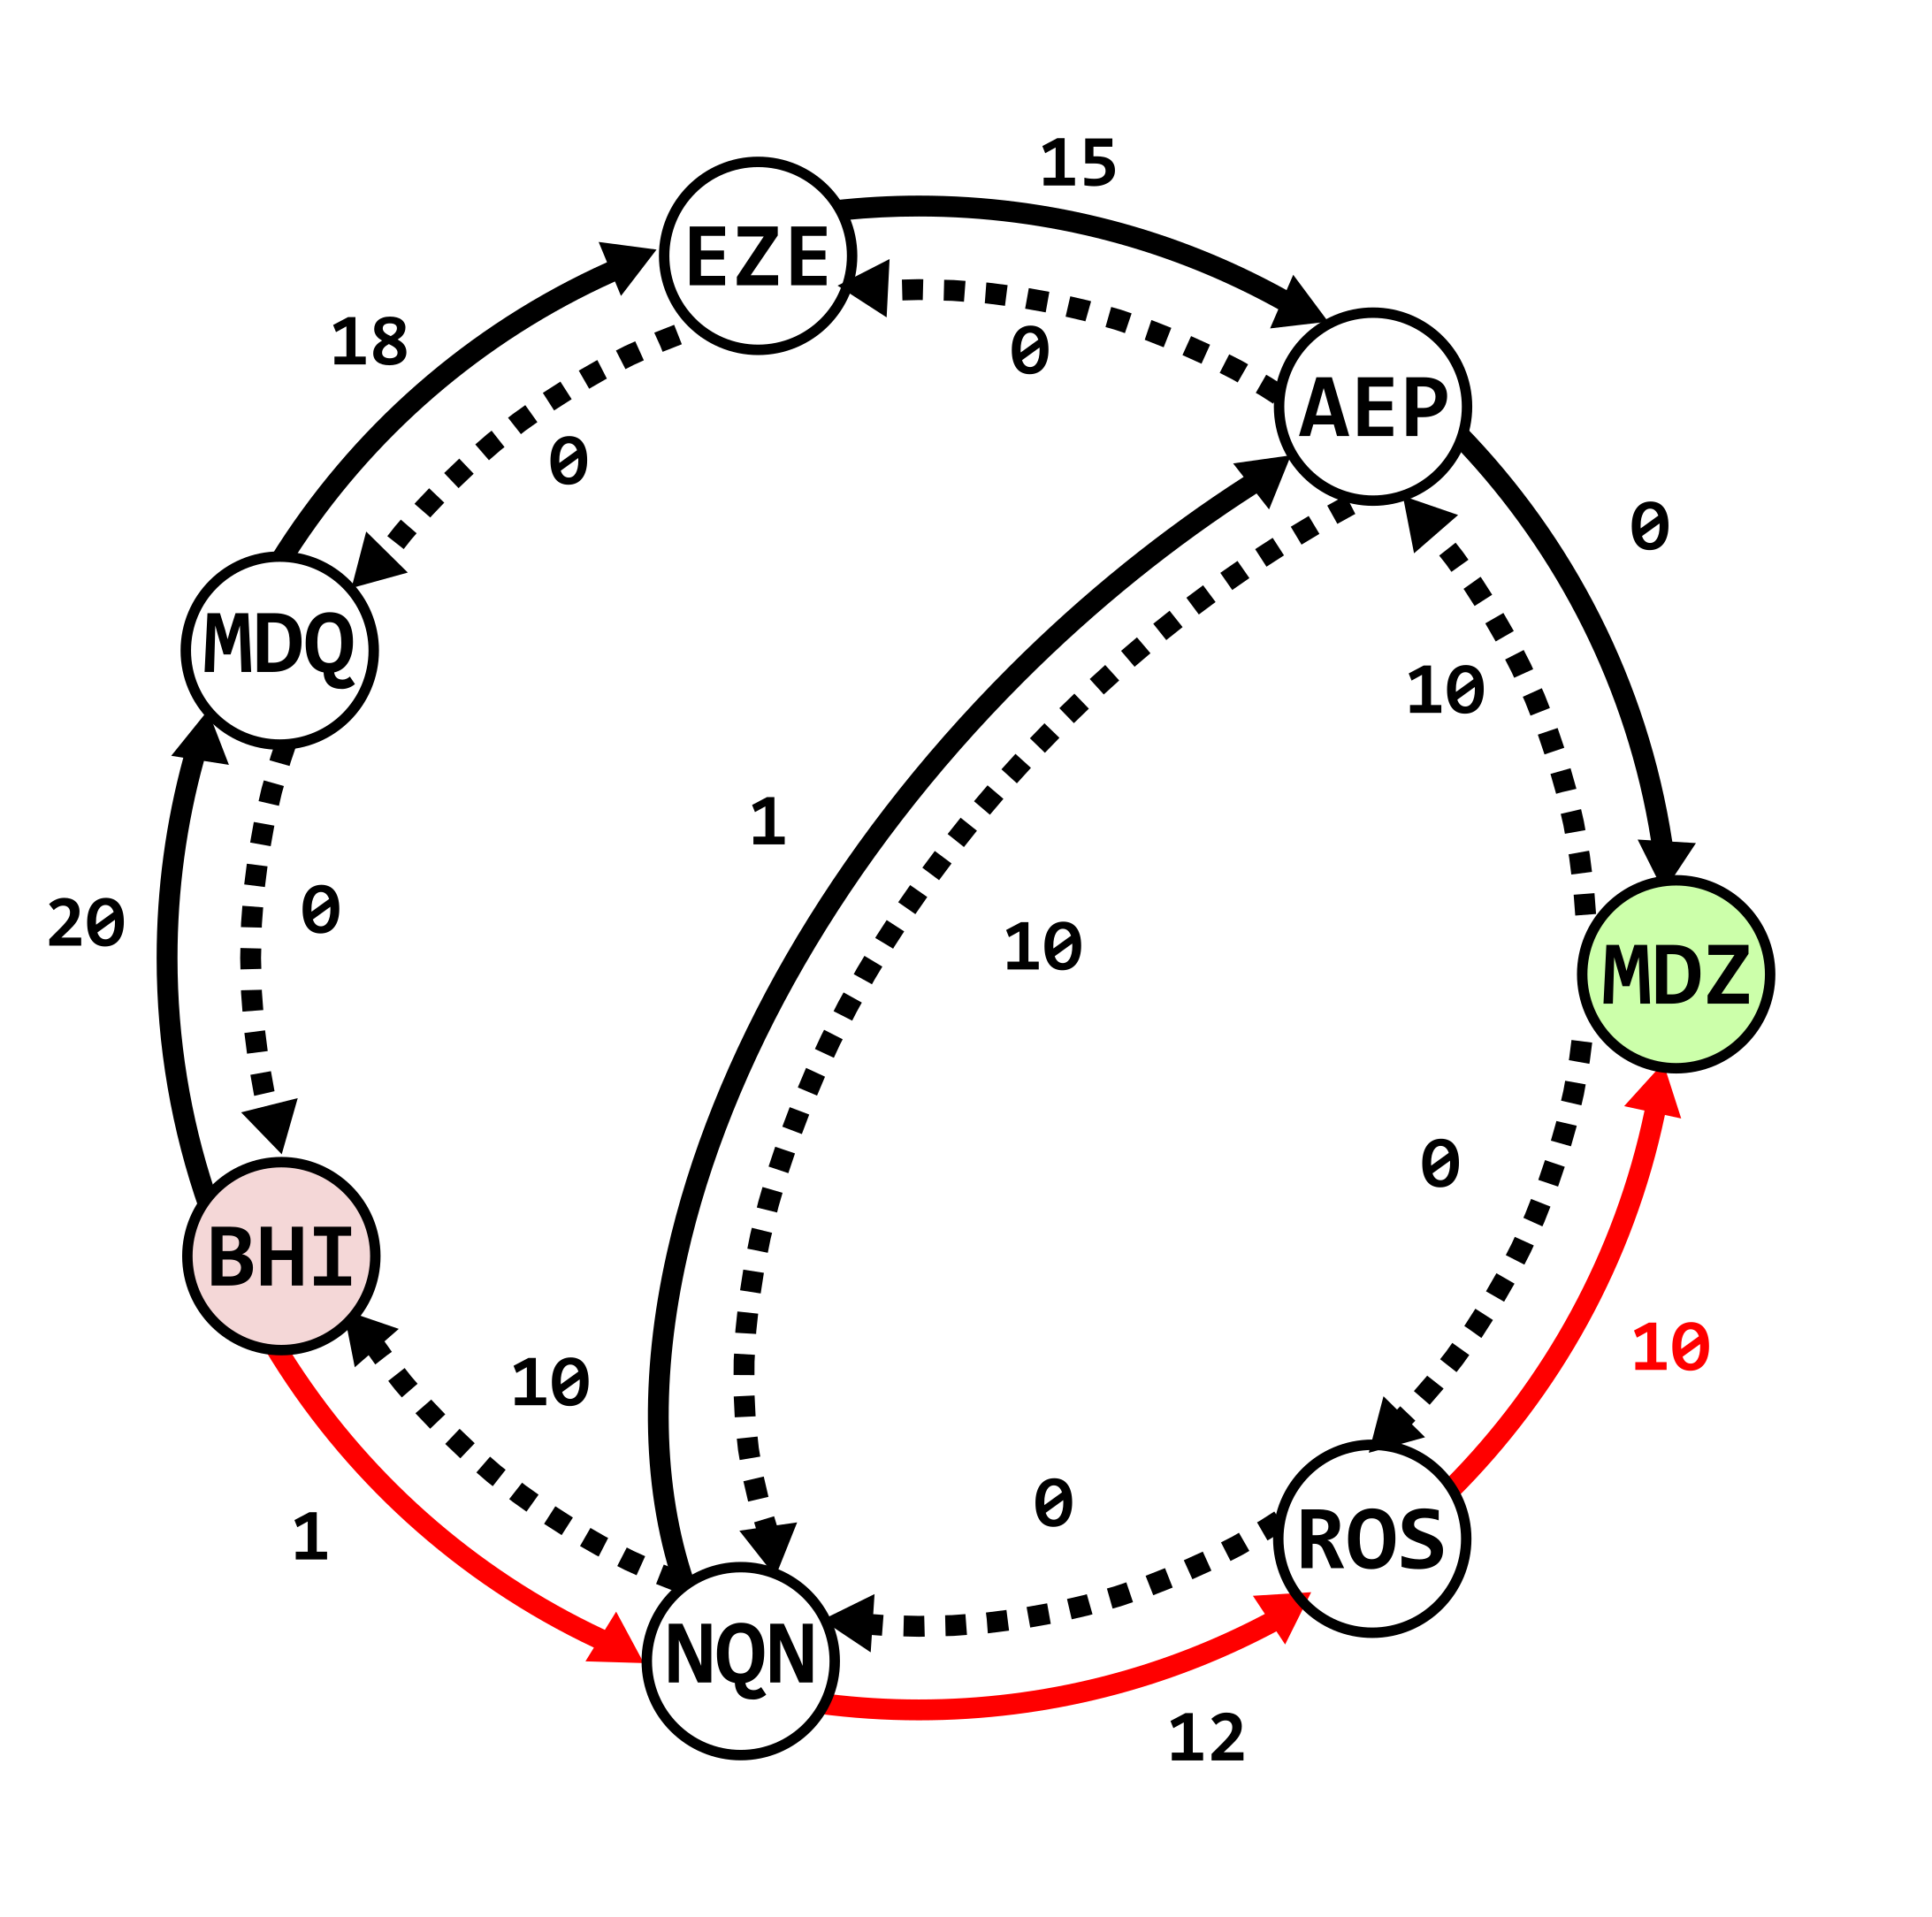
\includegraphics[width=0.4\linewidth,angle=0,origin=c]{out/ejA5.png}}
    \subcaptionbox
        {\label{fig:Vuelos6}\textbf{Aumentar:} Se vuelven a actualizar los valores. Ahora el flujo total queda en 11,
        al sumarle a los 10 anteriores, el último cuello. El arco que era cuello de botella queda en 0.}
        {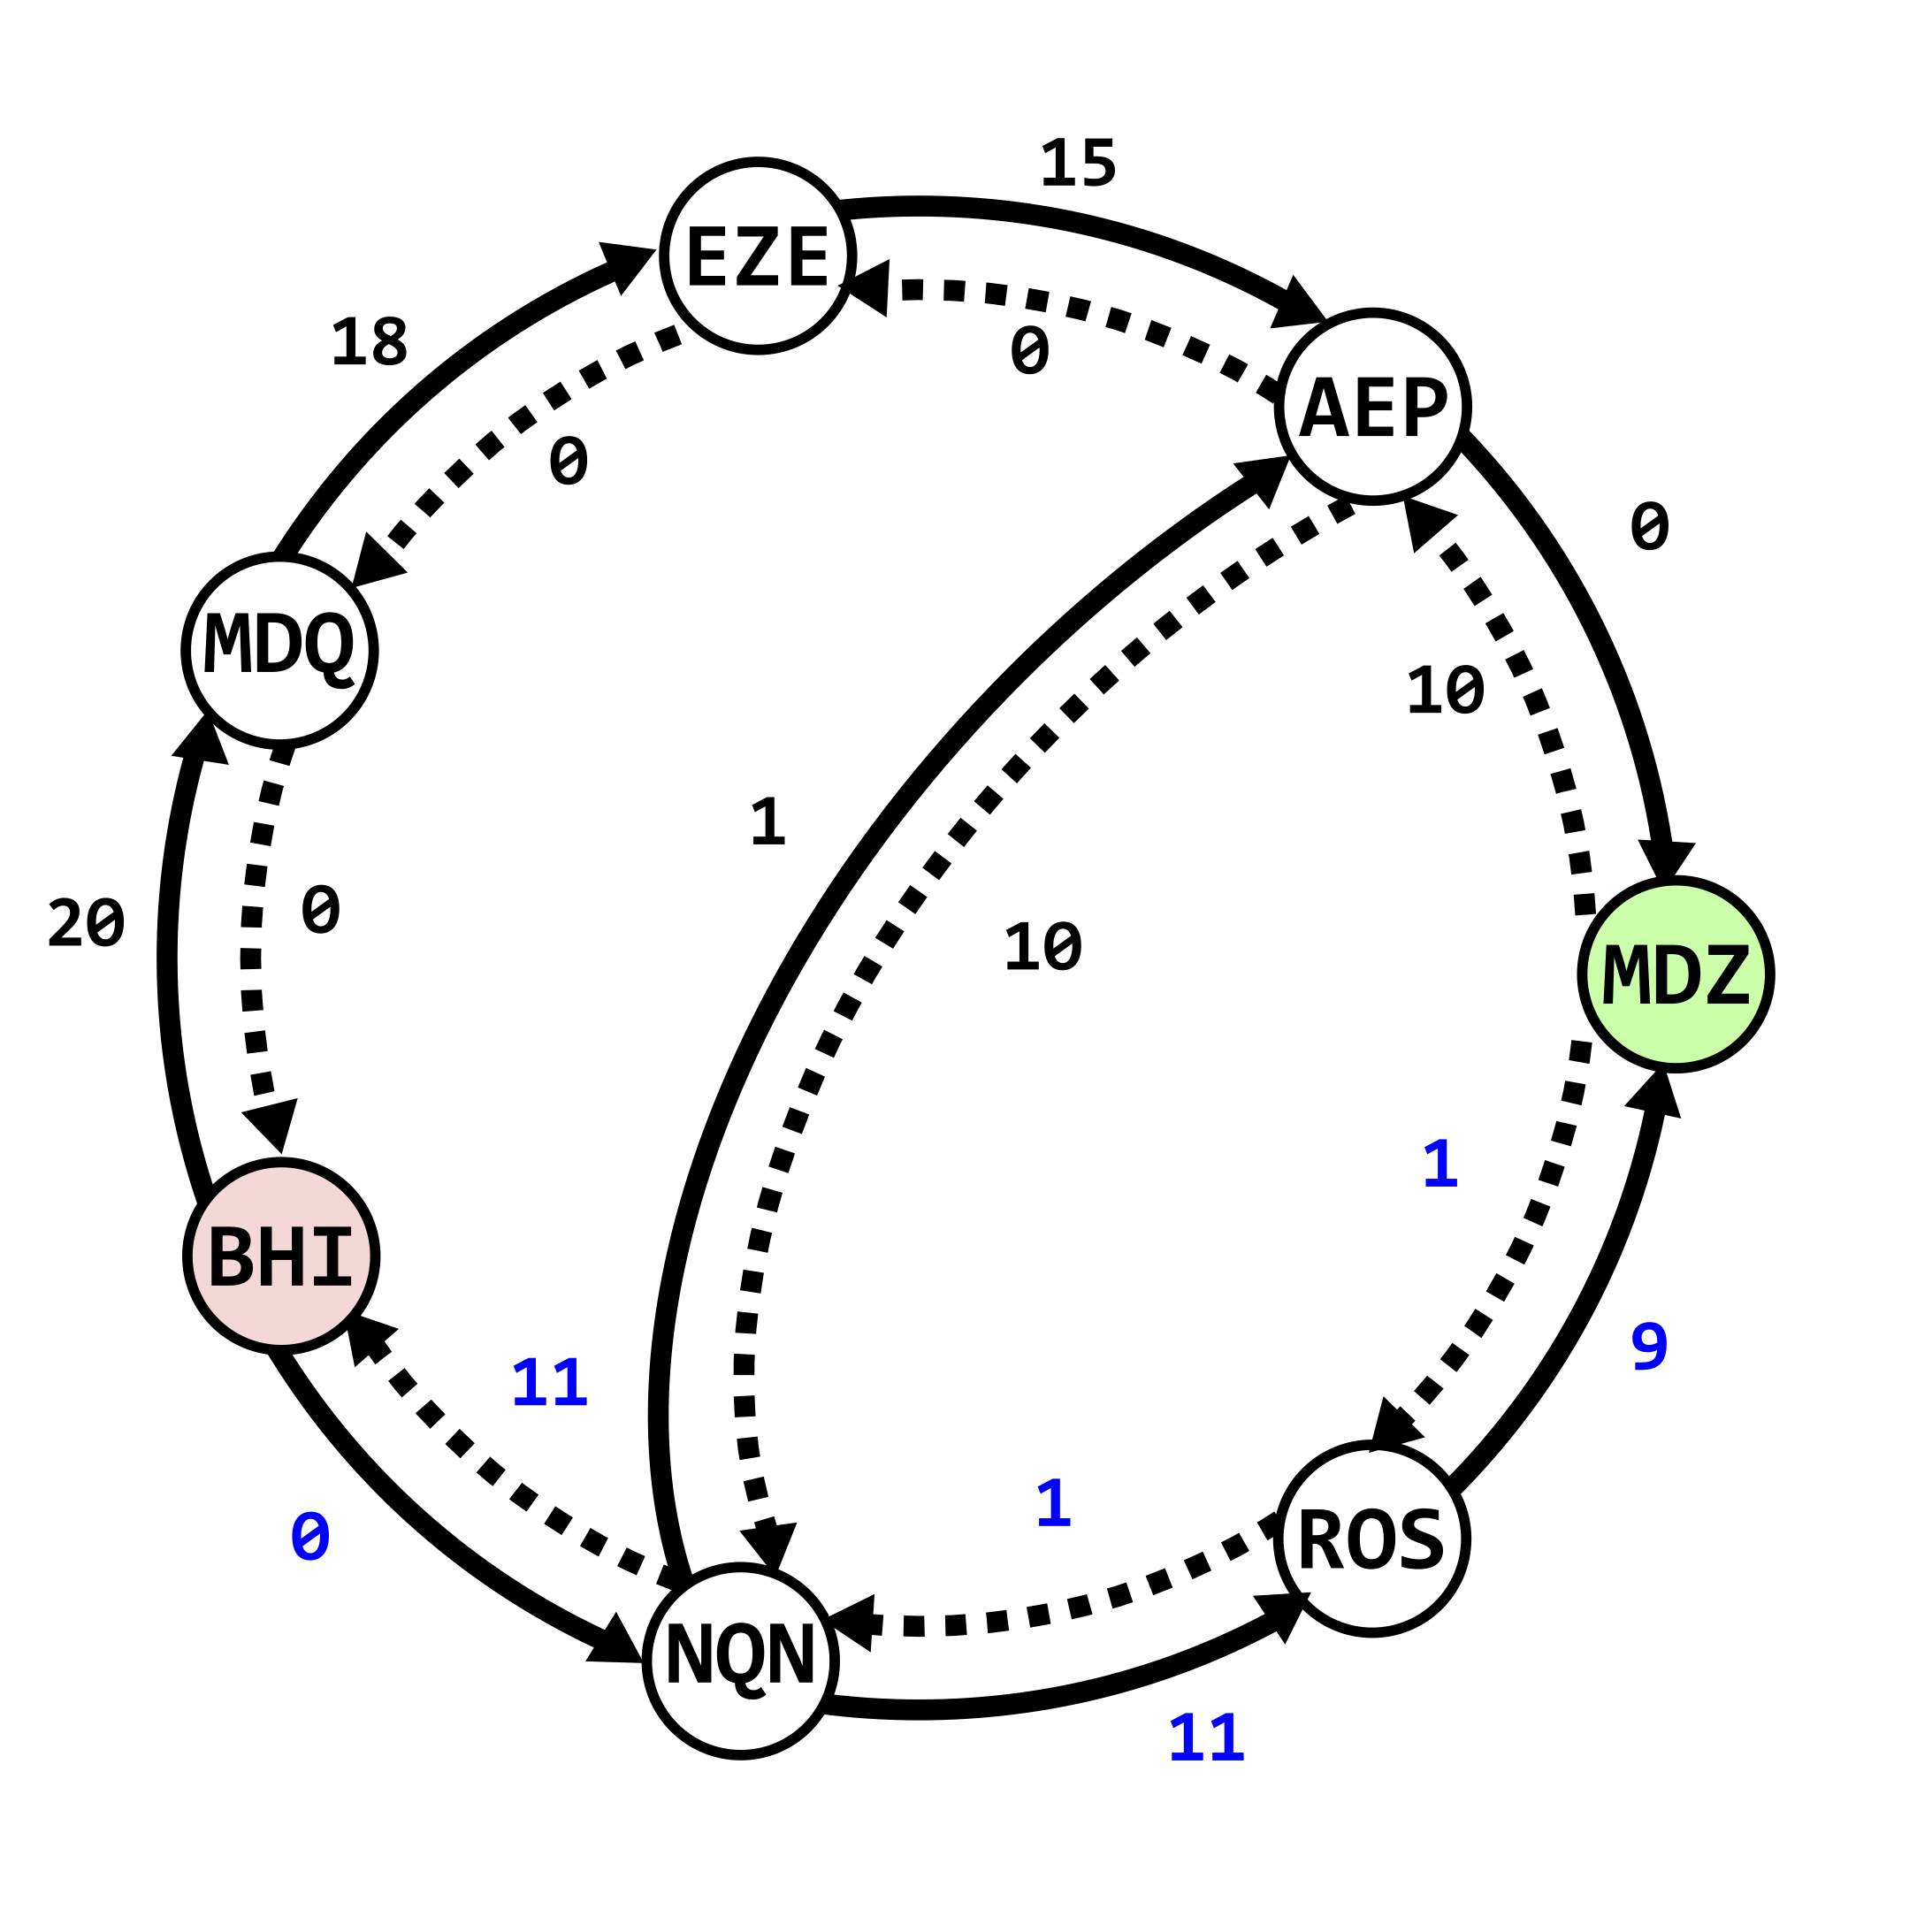
\includegraphics[width=0.4\linewidth,angle=0,origin=c]{out/ejA6.png}}
    \end{figure}
    \begin{figure}[H]
    %\ContinuedFloat
        \centering
    \subcaptionbox
        {\label{fig:Vuelos7}\textbf{BFS:} Como ahora $BHI\rightarrow NQN$ quedó saturado, el único camino disponible es
        el indicado en rojo. El cuello son los 9 de $ROS\rightarrow MDZ$.}
        {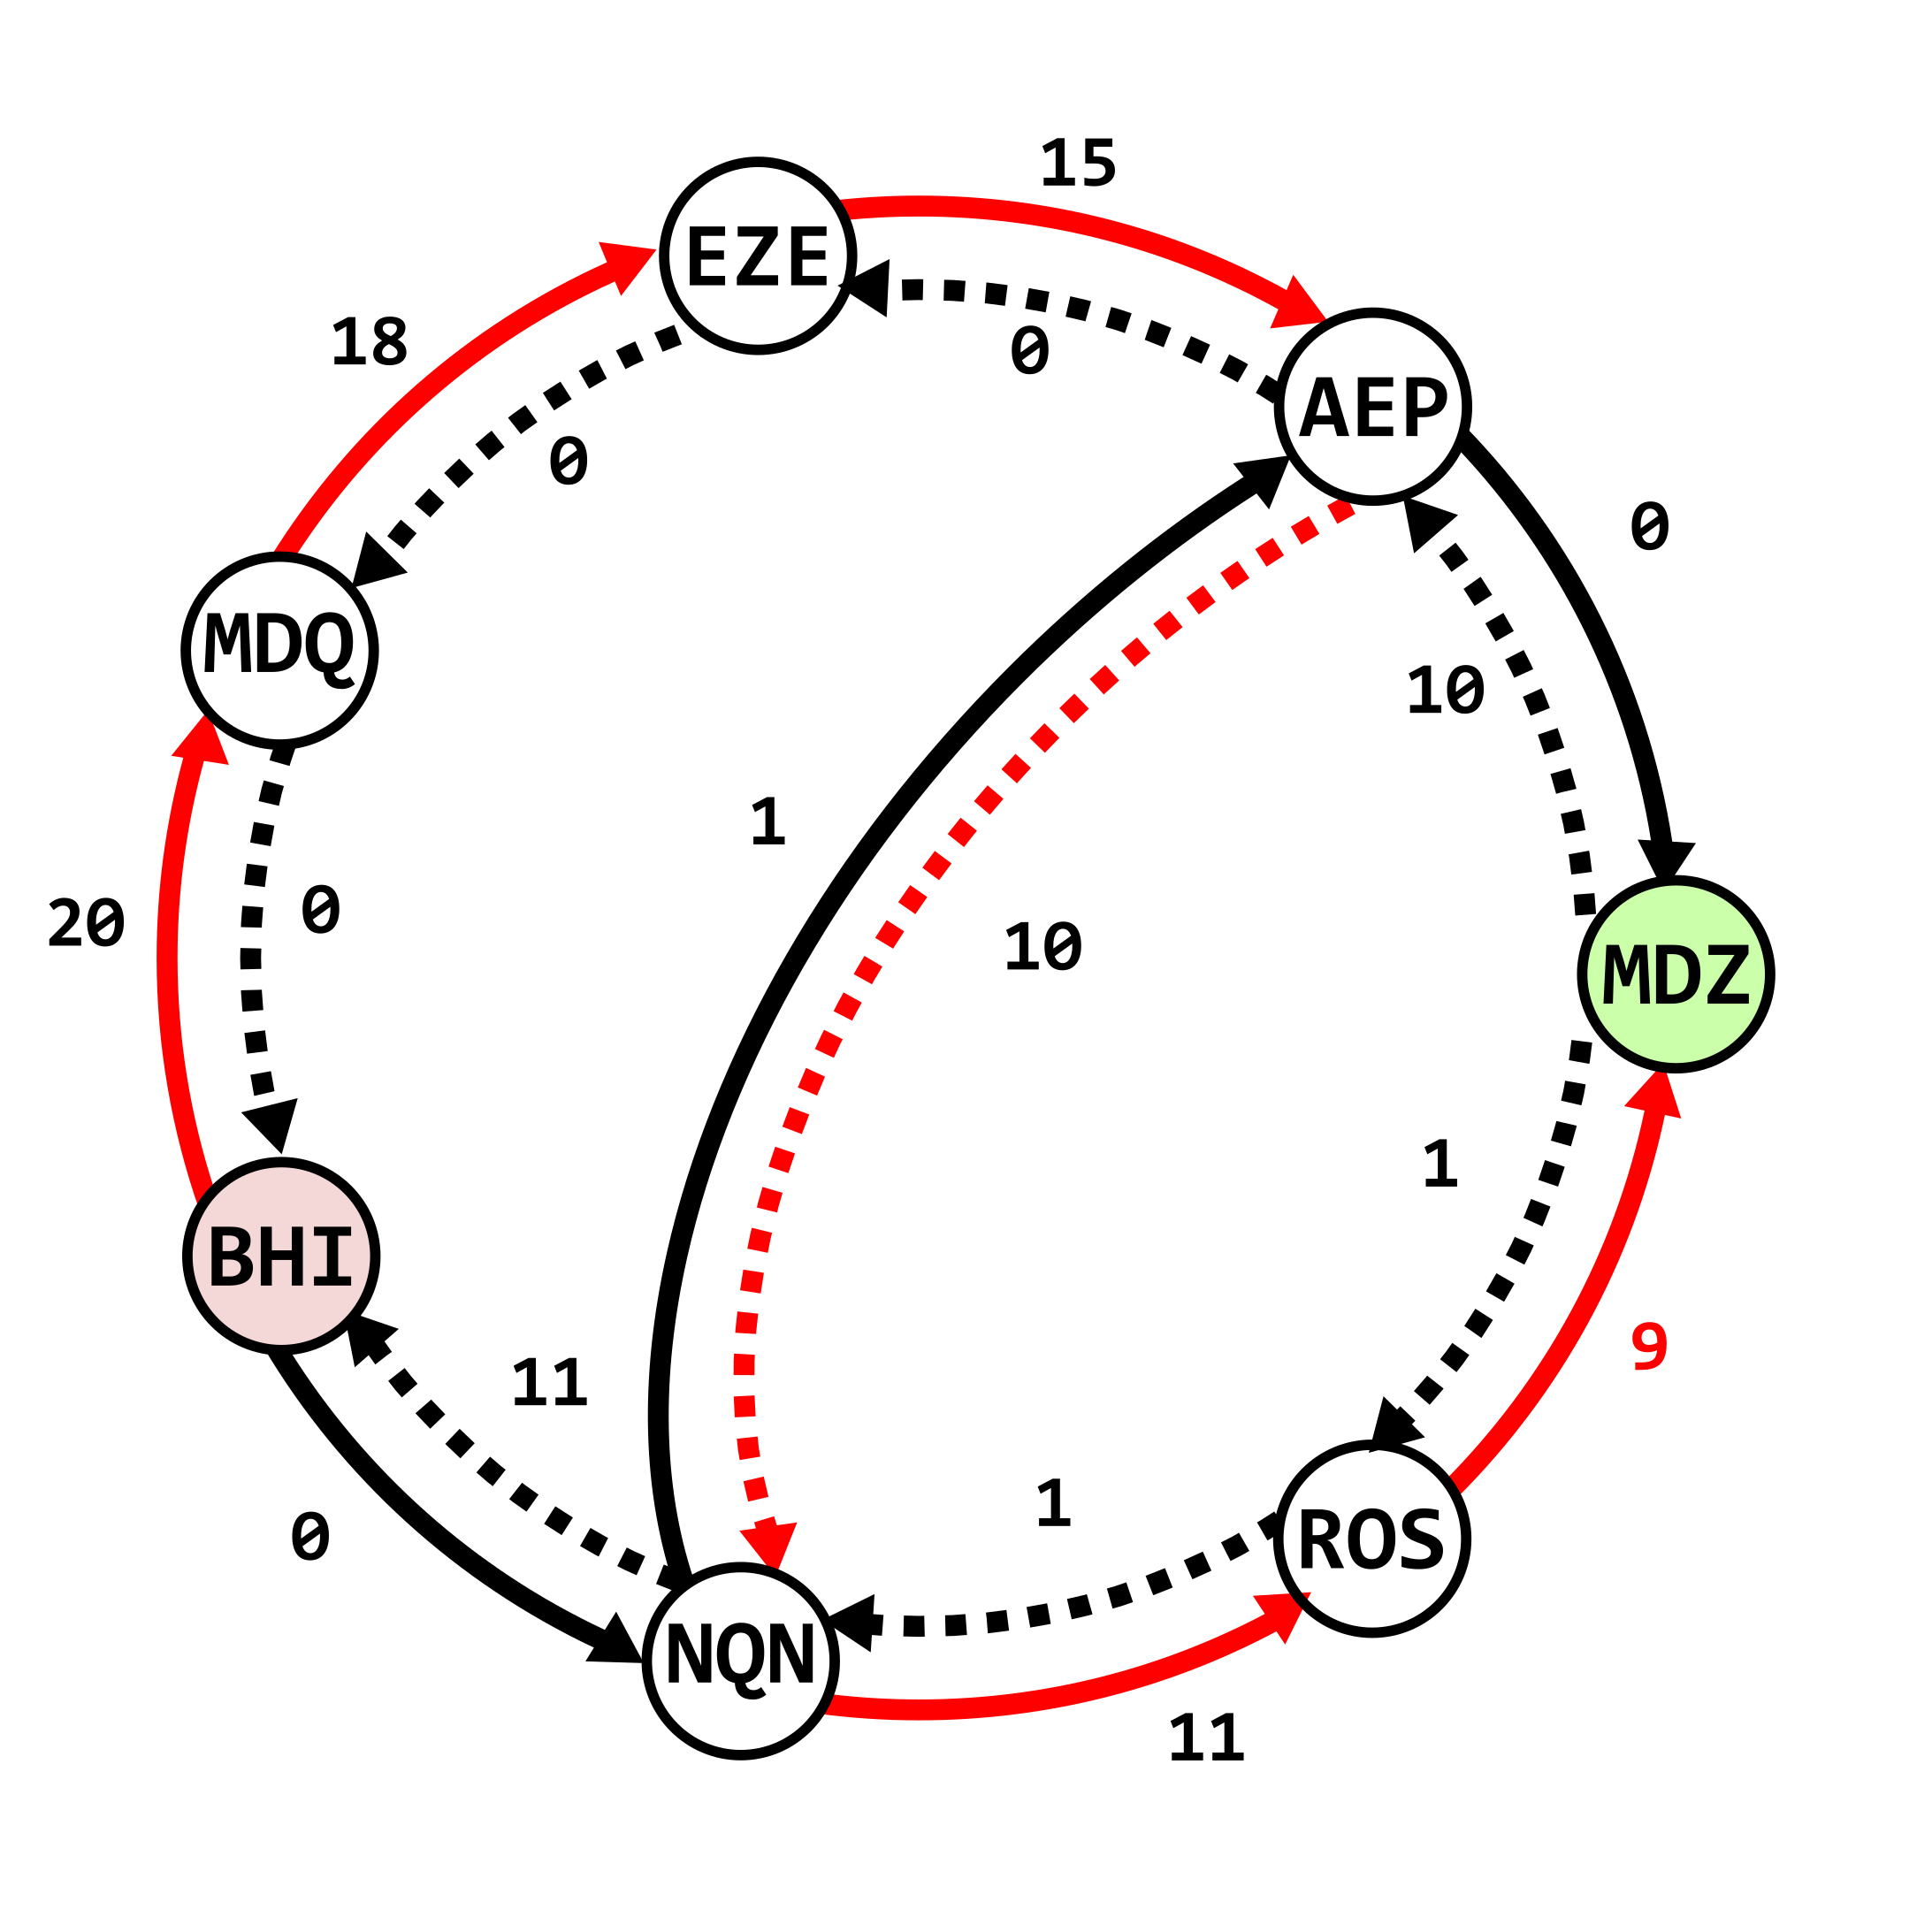
\includegraphics[width=0.4\linewidth,angle=0,origin=c]{out/ejA7.png}}
    \subcaptionbox
        {\label{fig:Vuelos8}\textbf{Aumentar:} Una vez actualizado en 9, también aumenta el flujo total en la misma cantidad
        llegando a 20. Aumentar el camnino de reversa implicó que 9 que llegaban a AEP por NQN ahora lo hacen por EZE; quedando
        esos 9 disponibles para ir a ROS.}
        {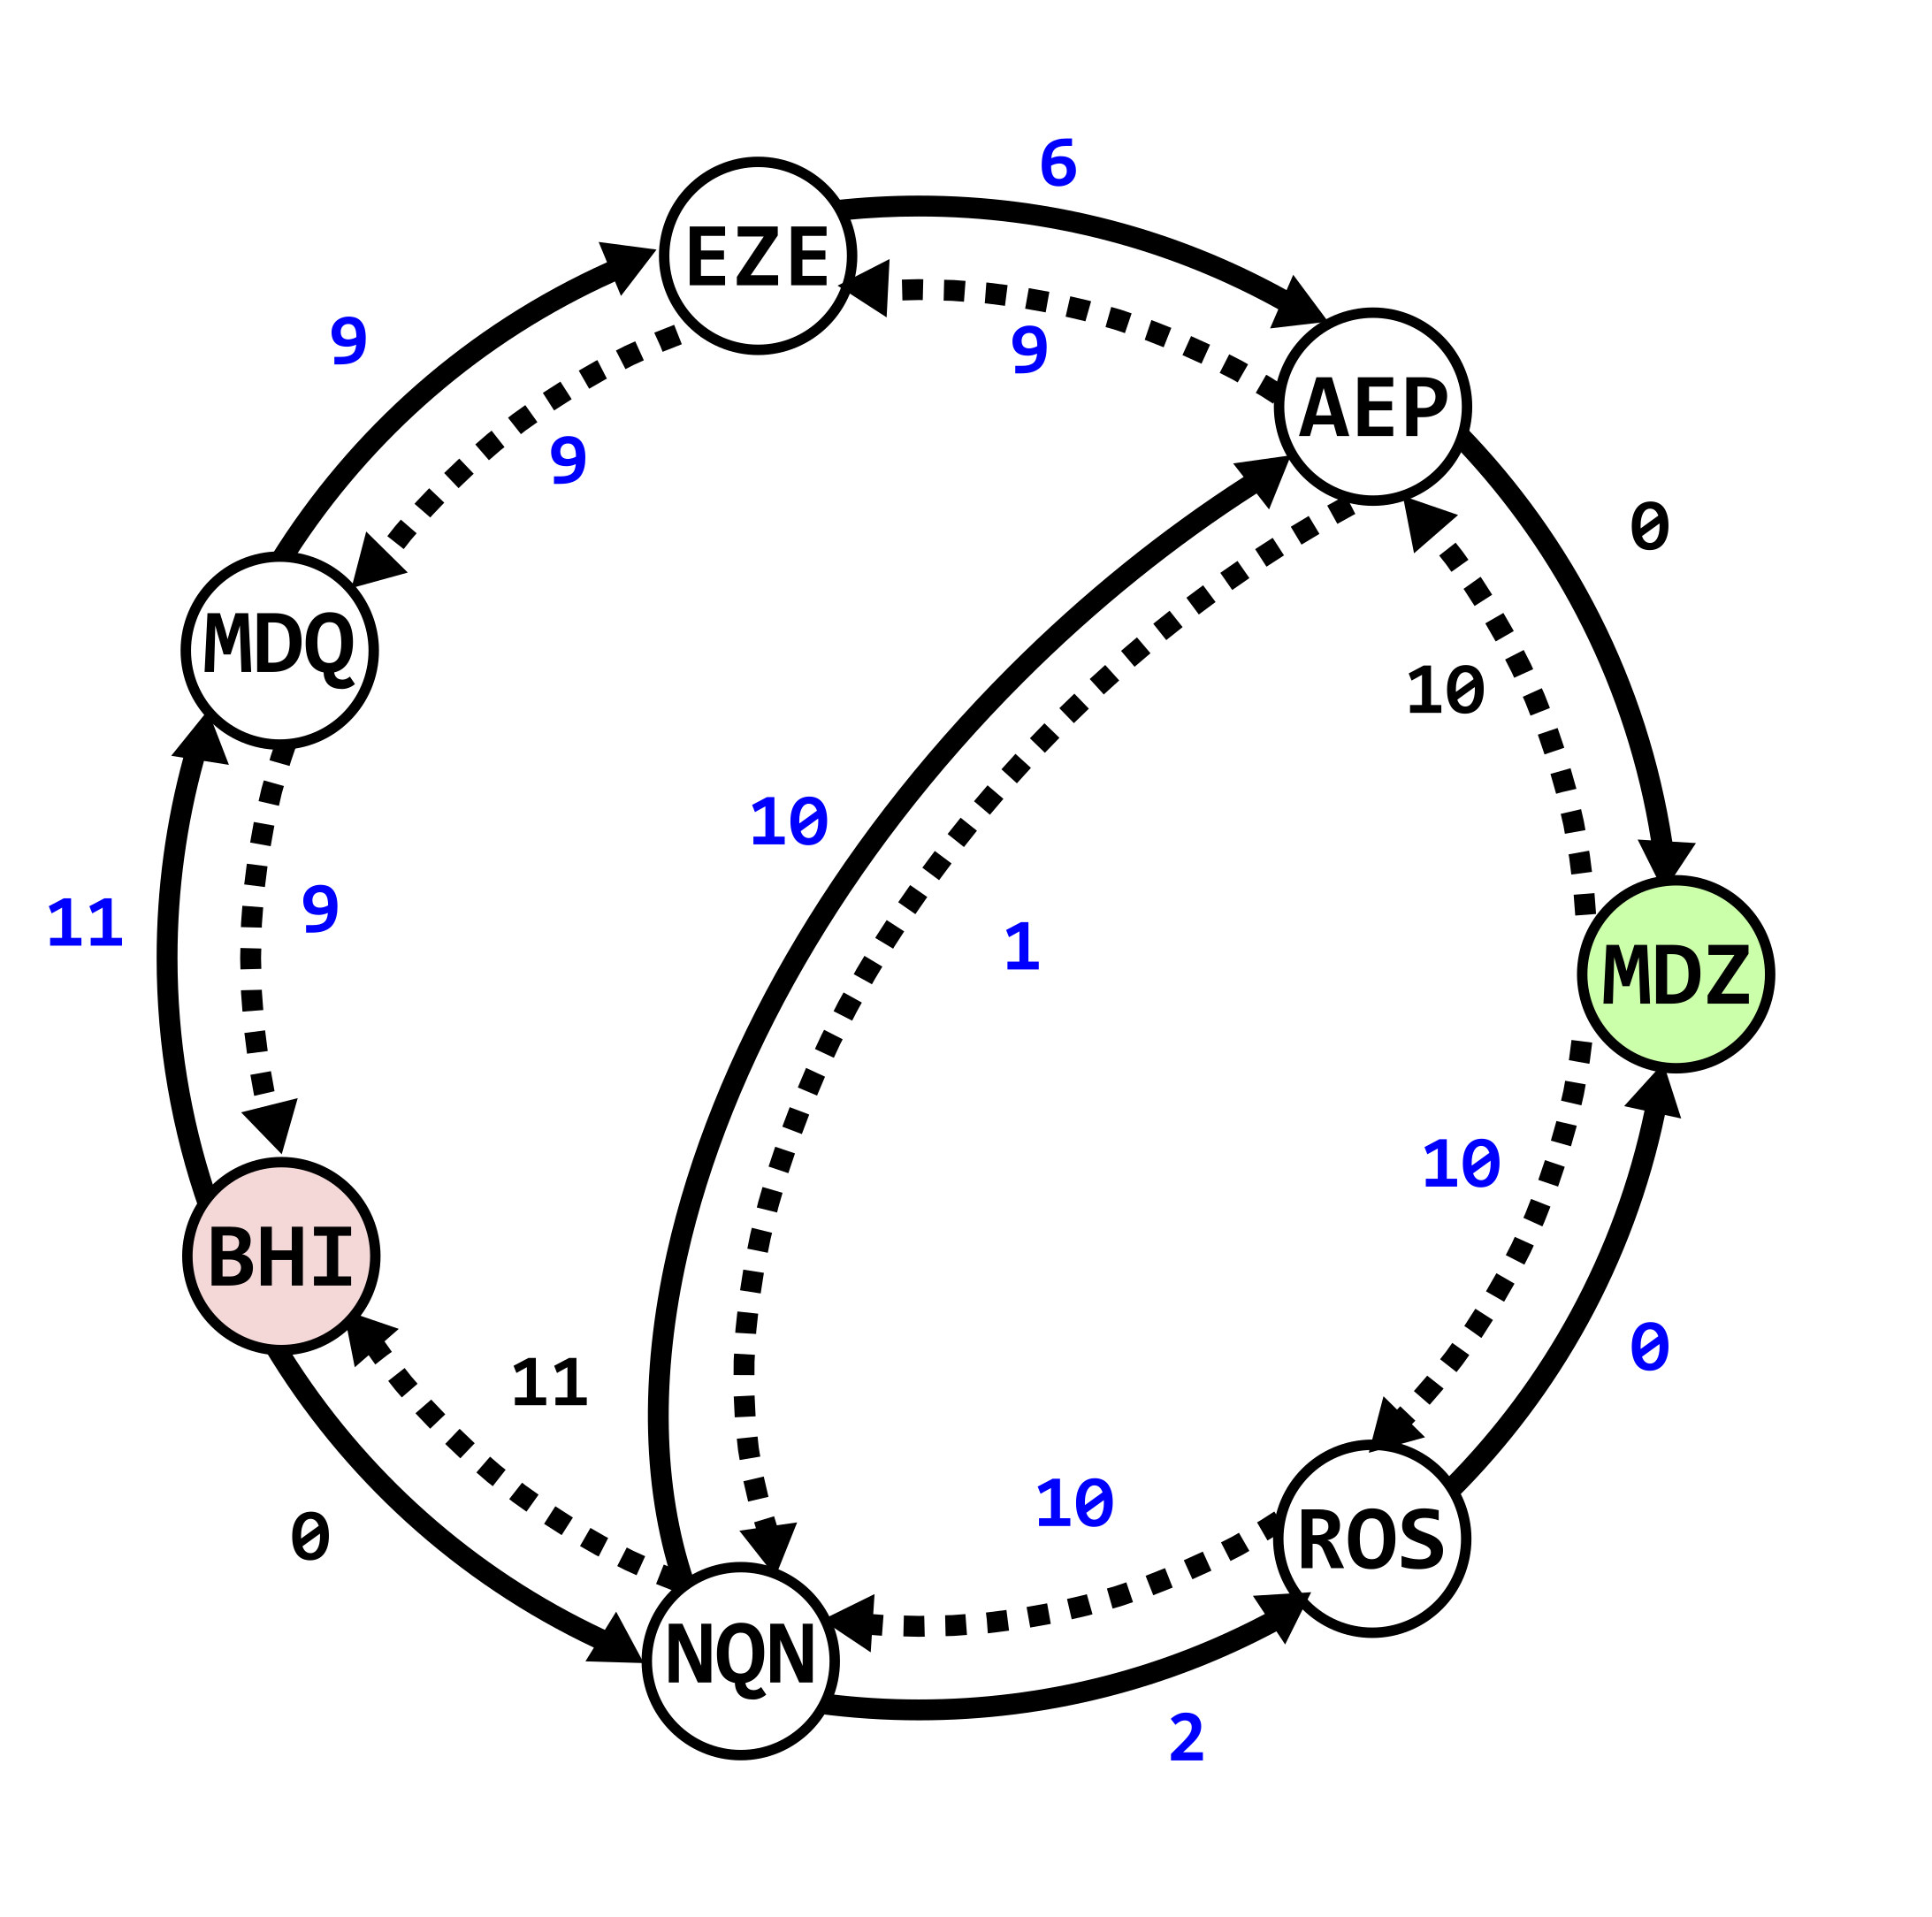
\includegraphics[width=0.4\linewidth,angle=0,origin=c]{out/ejA8.png}}
    \end{figure}
    \begin{figure}[H]
    %\ContinuedFloat
    \centering
    \subcaptionbox
        {\label{fig:Vuelos9}\textbf{Subgrupos y corte:} En azul nodos del subgrupo A (y los arcos por los que llegó).
        En verde el resto de los nodos, que quedan en subgrupo B. En rojo los arcos saturados que pertenecen al corte,
        y en bordó otros arcos saturados que pertenecen a un subgrupo.}
        {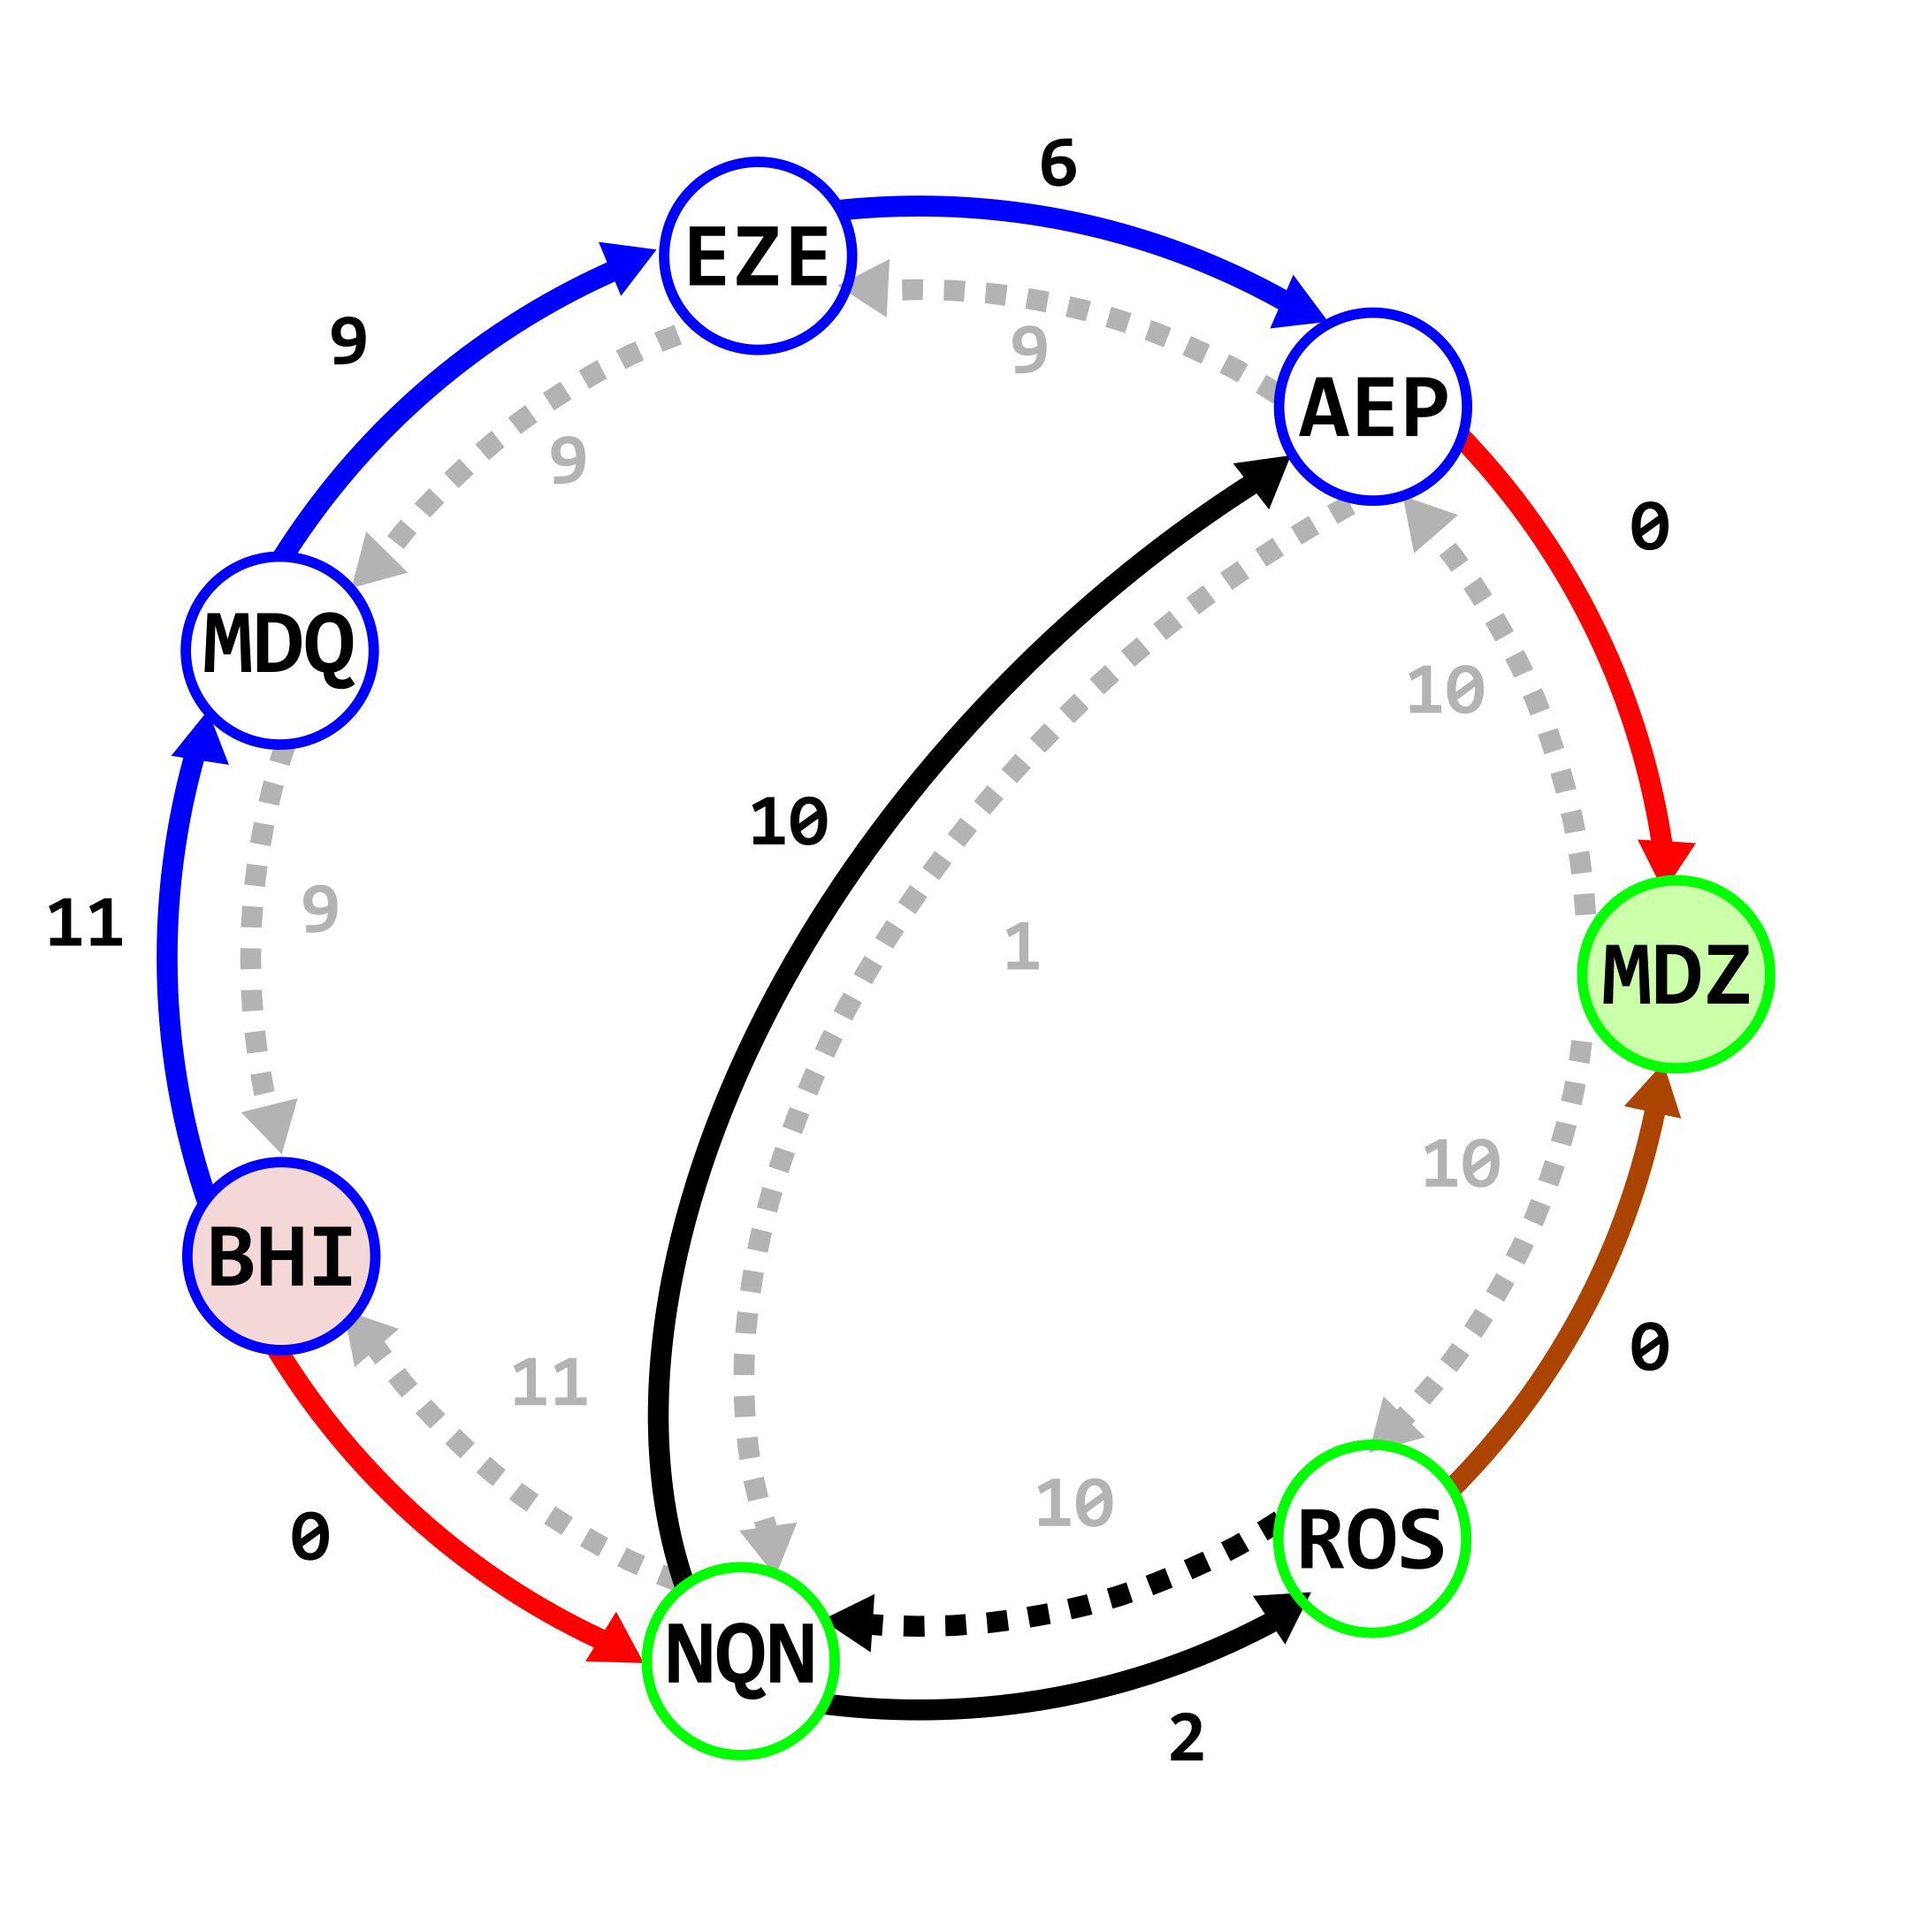
\includegraphics[width=0.4\linewidth,angle=0,origin=c]{out/ejA9.png}}
    \subcaptionbox
        {\label{fig:Vuelos10}\textbf{Reconversión:} Una vez resuelta la instancia como un problema de flujo, se convierte
        nuevamente en una instancia del problema original. En rojo los vuelos seleccionados, y la cantidad
        de pasajeros máxima es 20 (lo que era el flujo máximo).}
        {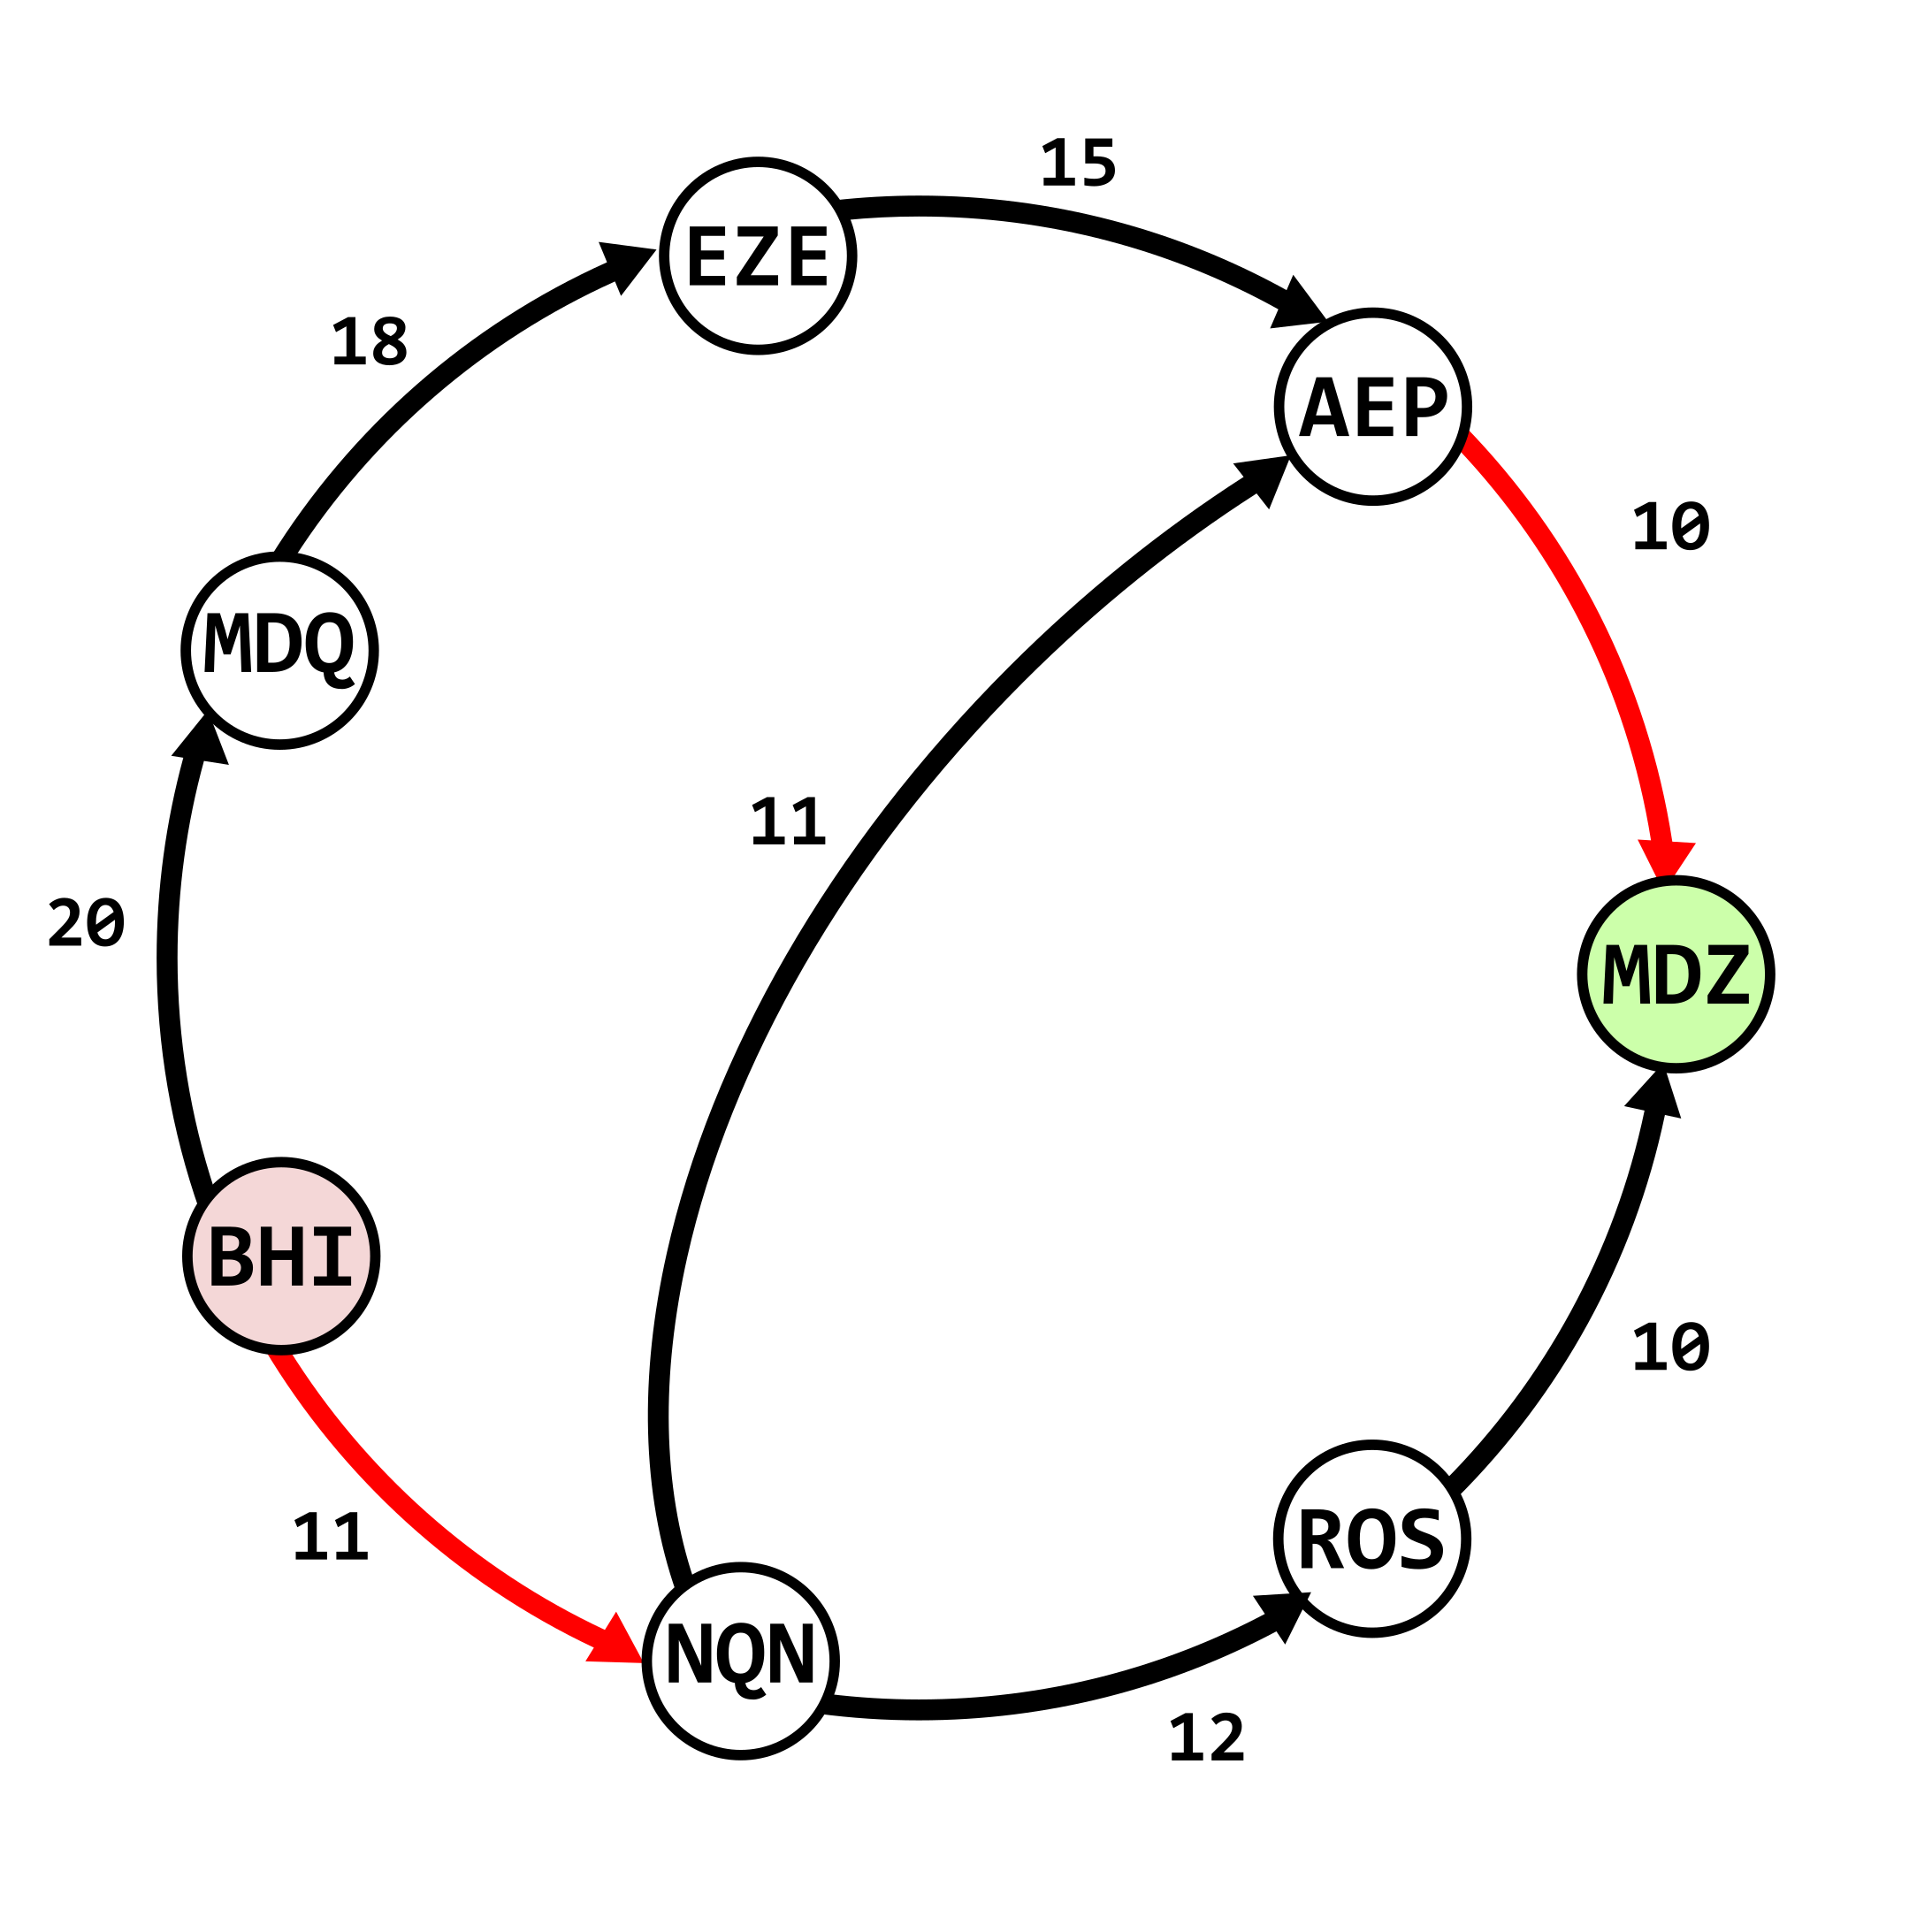
\includegraphics[width=0.4\linewidth,angle=0,origin=c]{out/ejA10.png}}
\end{figure}

% FIN DEL DOCUMENTO (SECCIÓN P1.1)
% NO BORRAR POR ACCIDENTE NI ESCRIBIR COSAS ABAJO
\end{document}